\chapter{Experimental Results and Evaluations}
\label{chap:k3}

\cref{sec:Materials} provides information about input dataset and the applied preprocessing steps. 

evaluation procedure
%The distance between the LIDAR points and the generated DSM are computed and evaluated statistically
%To evaluate the influence of the over-counting correction and MGM
%cost aggregation independently, two evaluations were performed


In \cref{sec:sd}, the correctness of the derived model is firstly verified by using simulation data without adding errors in the simulated measurements yet some biases are added in the initial values of the unknowns.

Dashed lane-lines reconstruction is presented in \cref{sec:td-short}. % 5 set of dashed lane line data
% show the differences with DSM profile
In long lane-lines reconstruction cases

%%%%%%%%%%%%%%%%%%%%%%%%%%%%%%%%%%%%%%%%%%%%%%%%%%%%%%%%
\section{Materials}
\label{sec:Materials}

\paragraph{Aerial Images}
For real-time mapping applications during disasters, mass events and traffic monitoring scenarios, the German Aerospace Center (DLR) has developed a new optical sensor system-- the 4k system-- on a helicopter from DLR. The oblique aerial images used in this work are acquired from a Canon EOS 1D-X camera, one of the three non-metric cameras in the 4k system, with an oblique viewing angle $\tau$ of 15$\degree$. The image data sets used in this work were acquired in around 500m flying height $H_{flight height}$ above ground, which leads to a GSD of ~7cm. % data of acquisition, number of images, length of flight strips,…->maybe in chapter “Experiments?

An example aerial image is shown in \cref{fig:OriImg}. \cref{tab:CameraProperties} lists the properties of this camera, and \cref{tab:SensorViewingGeometry} provides the viewing geometry information.


\begin{table}%[!h]
  \centering
  \begin{tabular}{ll}
  \toprule
                                      {} & \textbf{Canon EOS 1D-X} \\
  \midrule
  Lenses                          & Zeiss Makro Planar 2/50\\
  \\[-1em]
  Sensor / Pixel size             & Full frame CMOS / 6.944 \textmu m\\
  \\[-1em]
  \multirow{2}{*}{Image size}     & 5184$\times$3456 pixel, ratio 3:2\\
                                  & (17.9 MPix)\\
  \\[-1em]
  ISO                             & 100--204800\\
  \\[-1em]
  max. frame rate / max. images   & 14 fps/ 180 images\\
  \\[-1em]
  Exposure time                   & 30 s -- 1/8000 s\\
  \\[-1em]
  Data interface                  & LAN (EDSDK software interface)\\
  \bottomrule
  \end{tabular}
  \caption{Properties of the oblique camera }
  \label{tab:CameraProperties}
%\end{table}
\vspace{1cm}
%\begin{table}%[!h]
  \centering
  \begin{tabular}{lll}
  \toprule
                         & \textbf{RGB, 50mm lens} \\
  \midrule
  Viewing directions     & $\pm$15$\degree$\\
  \\[-1em]
  \multirow{2}{*}{FOV}   & $\pm$34$\degree$ across strip,\\
                         & $\pm$13$\degree$ along strip\\
  \\[-1em]
  Coverage @500m         & 780 m $\times$ 230 m\\
  GSD      @500m         & 6.9 cm (nadir)\\

  \bottomrule
  \end{tabular}
  \caption{Viewing geometry}
  \label{tab:SensorViewingGeometry}
\end{table}

The images used in this work are acquired with a special flight configuration at both sides of the motorway which guarantees a continuous stereo view perpendicular to the lane marking direction.\footnote{The classical photogrammetric approach on flight planning is to have several straight flight lines which cover the whole motorway in a stereo view. This would be possible in this project yet would require more flight costs and would produce many more images.} This is realized by flying at the right-hand side with respect to flying direction along the motorway, with the left oblique camera looking left-down to the motorway, in both forward and backward trip. The flight configuration is shown in \cref{fig:FlightTrajectory} on the Google Earth platform.

Besides, the forward overlap is around 70\%, and all the lane markings are covered by both strips, whereas the side overlap depends on the distance of flight strips, which are a result of the pilots navigation ability and other influences, like wind. Nevertheless, the motorway in its entire width was covered by the two flight strips. Altogether, this results in approximately 8-image coverage in road areas. 

\begin{figure}%[!h]
  \centering
  \subfloat[]{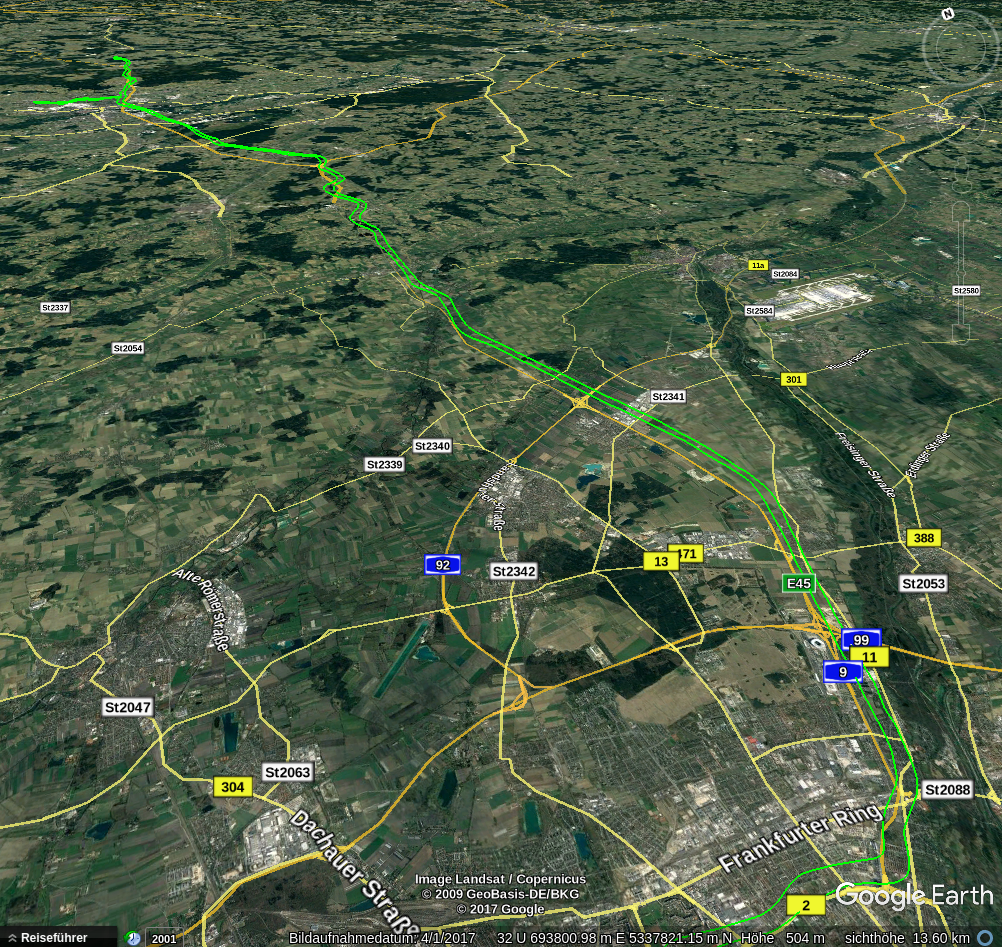
\includegraphics[height=0.45\textwidth]{FlightTrajectory5.png} \label{fig:trajectory1}}
  \subfloat[]{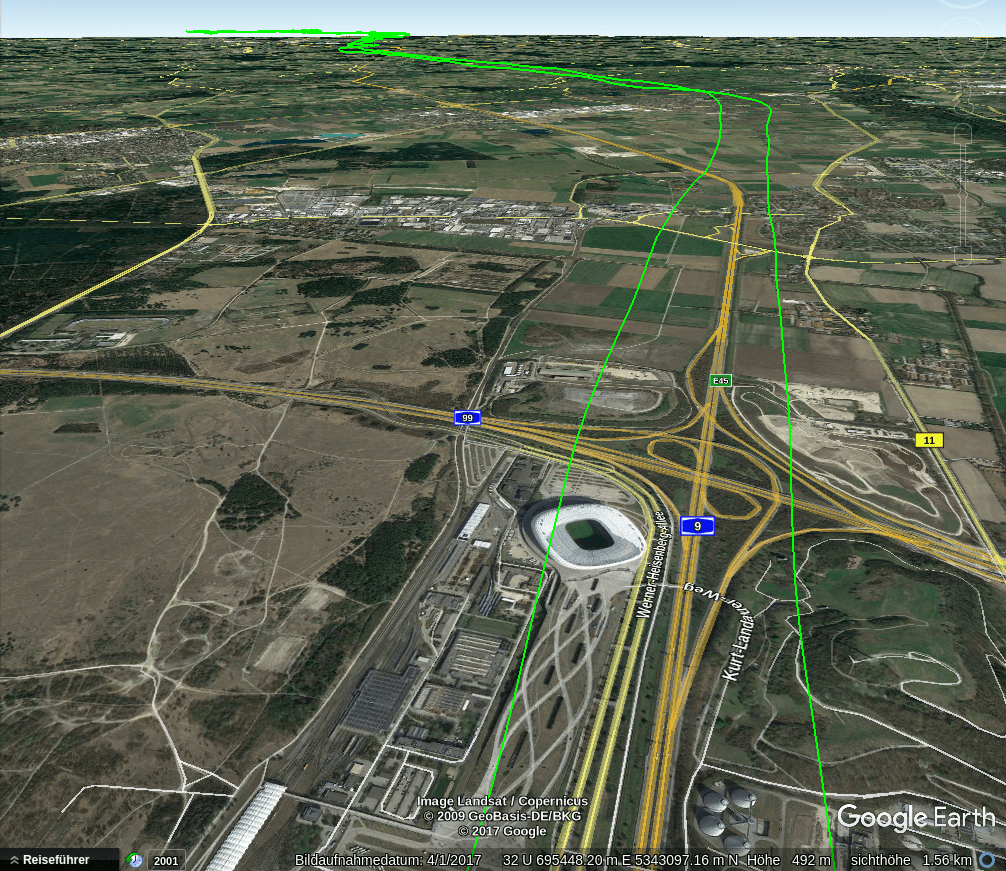
\includegraphics[height=0.45\textwidth]{FlightTrajectory3.png} \label{fig:trajectory2}}
  \caption{\small Flight trajectory of DLR helicopter visualized on the Google Earth platform. The green polyline shows the flight trajectory. \textit{Source: \textbf{Google Earth} 04/01/2017}}
  \label{fig:FlightTrajectory}
\end{figure}


\paragraph{Exterior and Interior Orientations}
The \gls{eo} of the images are directly measured by a GNSS/Inertial system IGI IId.% Missing: specification of the system, improvements by SAPOS correction,….
The EO parameters are then refined by a self-calibrating bundle adjustment. The accuracies of the exterior orientation (EO) parameters are shown in \cref{tab:EOaccuracy}. The calibrated \gls{io} parameters and their accuracies are shown in \cref{tab:IOaccuracy}. To provide an overall quality on the interior orientations: from the calibration result of interior orientations (involving lens distortion), the residuals appear non-systematic and the biggest residual $r_{max, IO}$ is around $1$ pixel.

To judge the influence of exterior and interior parameters on positioning accuracy in object space, the maximum values for each component based on the flight configuration was calculated.
The quality of interior and exterior orientation parameters set would have a maximum impact in object space for around $16.5$ [cm] in X,Y-direction:
\begin{itemize}
      \item caused by inaccurate camera position: 
      \item [] $\sqrt{\sigma_{north}^2+\sigma_{east}^2}=\sqrt{0.055^2+0.035^2}\approx0.065$ [meter]
      \item caused by inaccurate camera attitude:
      \item [] $\tan(\sqrt{\sigma_{roll}^2+\sigma_{pitch}^2})\times H_{flight height}\times\dfrac{1}{\cos^2\tau}$
      \item [] $=\tan(\sqrt{0.002^2+0.002^2})\times 500\times\dfrac{1}{\cos^215\degree}\approx0.026$ [meter]
      \item caused by inaccurate Interior Orientations:
      \item [] $r_{max, IO}\times GSD\times\dfrac{1}{\cos^2\tau}=1\times0.069\times\dfrac{1}{\cos^215\degree}\approx0.074$ [meter]
\end{itemize}
and around $9.4$ [cm] in Z-direction:
\begin{itemize}
      \item caused by inaccurate camera position:
      \item [] $\sigma_{altitude}\approx0.069$ [meter]
      \item caused by inaccurate camera attitude:
      \item [] $\tan(\sqrt{\sigma_{roll}^2+\sigma_{pitch}^2})\times H_{flight height}\times\dfrac{\sin\tau}{\cos\tau}$
      \item [] $=\tan(\sqrt{0.002^2+0.002^2})\times 500\times\dfrac{\sin15\degree}{\cos15\degree}\approx0.007$ [meter]
      \item caused by inaccurate Interior Orientations:
      \item [] $r_{max, IO}\times GSD\times\dfrac{\sin\tau}{\cos\tau}=1\times0.069\times\dfrac{\sin15\degree}{\cos15\degree}\approx0.018$ [meter]
\end{itemize}

The above information tells the positioning accuracy in object space with measurements on a single image. With corresponding measurements from multiple stereo views, which allows the intersection of multiple  rays, the positioning accuracy is expected to be improved for being overdetermined.

\begin{table}%[!h]
    \centering
    \begin{tabular}{ll|ll}
    \toprule
    position accuracies  &[meter]  & attitude accuracies & [degree]\\
    \midrule
    $\sigma_{north}$     & $0.055$ & $\sigma_{Roll}$  & $0.002$\\
    $\sigma_{east}$      & $0.035$ & $\sigma_{Pitch}$ & $0.002$\\
    $\sigma_{altitude}$  & $0.069$ & $\sigma_{Yaw}$   & $0.005$\\
    \bottomrule
    \end{tabular}
    \caption{Accuracies of Exterior Orientations}
    \label{tab:EOaccuracy}
%\end{table}
\vspace{1cm}
%\begin{table}%[!h]
    \centering
    \begin{tabular}{lr|lr|l}
    \toprule
    \multicolumn{2}{c|}{Interior Orientations}  & \multicolumn{2}{c|}{accuracies} & unit\\
    \midrule
    focal length $c$                       &   $0.051$ & $\sigma_c$      & $6.9\mathrm{e}{-7}$ & [meter]\\
    x coordinate of principal point $pp_x$ & $-42.259$ & $\sigma_{pp_x}$ & $0.167$             &[$\mu$m]\\
    x coordinate of principal point $pp_y$ & $115.384$ & $\sigma_{pp_y}$ & $0.799$             &[$\mu$m]\\
    \bottomrule
    \end{tabular}
    \caption{Interior Orientations and their accuracies}
    \label{tab:IOaccuracy}
\end{table}

\paragraph{\gls{dsm}}
For each pair of stereo images, a disparity map is generated using \gls{sgm} algorithm. With disparity's property of being inversely proportional to depth, the disparity maps can be used to derive the DSM. Since SGM is a kind of appearance-based matching, the SGM-generated DSM is noisy in lowly textured regions. 
%In most of the cases, a point in object space is covered by more than two aerial images, resulting in more than one disparity map. This leads to ambiguities on height decision during DSM generations.
%, and can be solved by simply taking the median value derived from disparity maps in odd number of disparity maps cases, and the value just lower than the median in even number cases. %This results in systematic errors of having lower height value in some parts of DSM.(The whole proof of this sentence is more complicated, I hope you will be not asked about this.)
Thus, the DSM will be used only for setting up the initial values of the work flow, and will not influence the final results of the 3D lane marking reconstruction.

The DSM has 20 cm grid spacing. \cref{fig:DSM} shows a part of the DSM. Standard deviations of the height value in this part of the DSM is shown in \cref{fig:DSMstd}. The number of stereo image pairs used for each part on the DSM is shown in \cref{fig:DSMnumber}.
% problem of higher noise at road surfaces
% Standard deviation not well visible. Maybe add number of images for this small part
\begin{figure}%[!h]
  \centering
  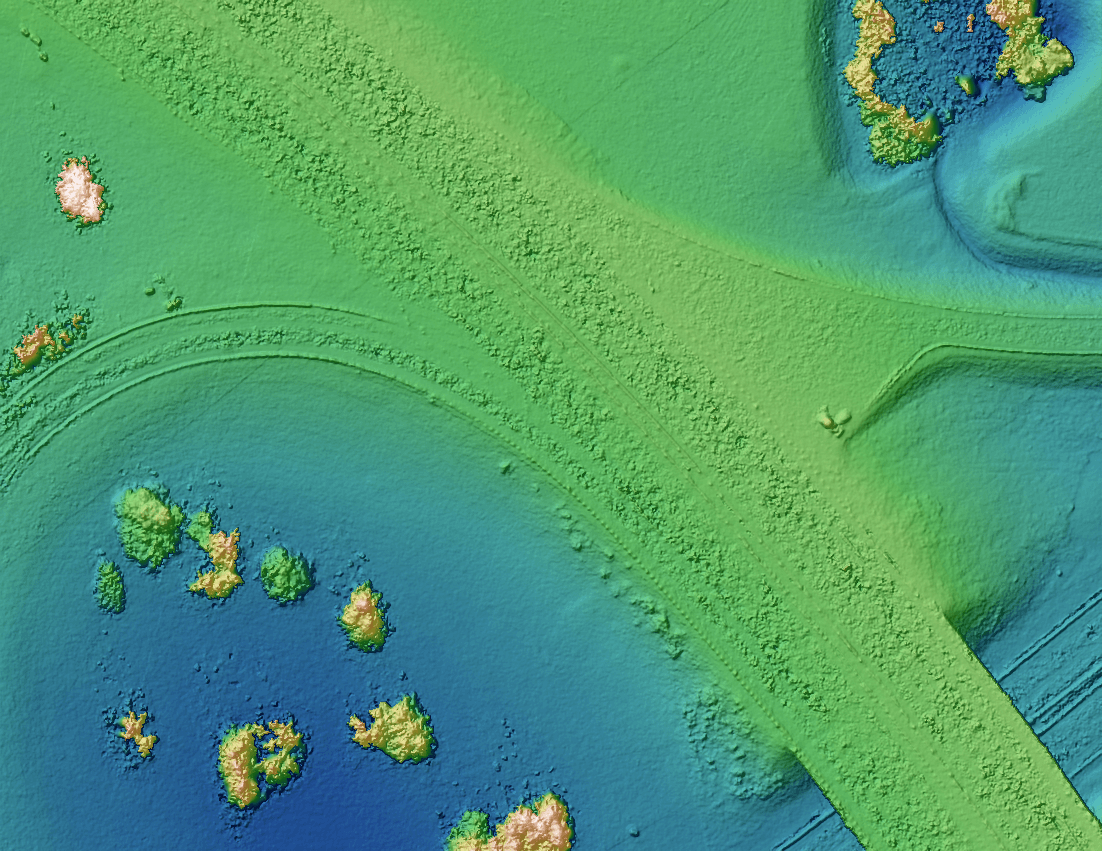
\includegraphics[width=0.8\textwidth]{DEM_A9_FINAL_PART_small_shaded.png}
  \caption{\small Part of the DSM in road area. It is noisy in the center of motorway.}
  \label{fig:DSM}
  \vspace{1cm}
  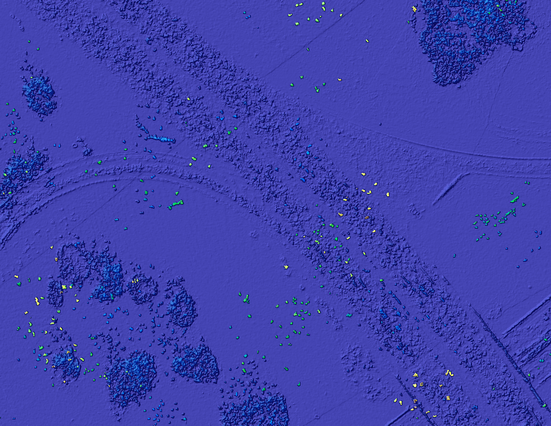
\includegraphics[width=0.8\textwidth]{DEM_A9_STD_small_terrain.png}
  \caption{\small Standard deviations of the height value of the DSM in road area. It has higher value in the center of motorway.}
  \label{fig:DSMstd}

\end{figure}

\begin{figure}%[!h]
  \centering
  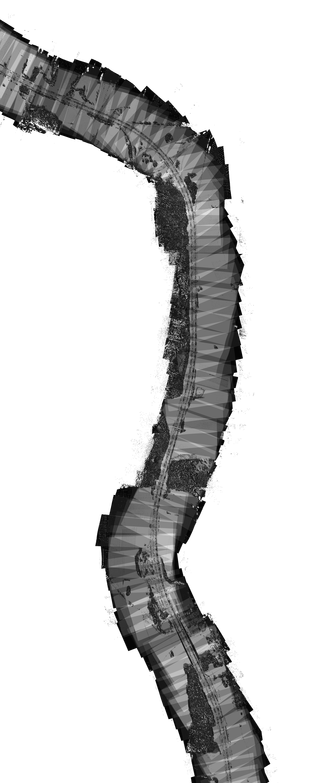
\includegraphics[width=0.5\textwidth]{DEM_A9_NUM_scaled_s.png}
  \caption{\small Distribution of stereo pairs used for DSM generation. Lighter color indicates more stereo pairs are used in that area. Maximum 27 stereo pairs are used for one pixel.}%%%%%%%%
  \label{fig:DSMnumber}
\end{figure}


\paragraph{Orthorectified Images}
The orthorectified images are processed using the DSM and the interior and exterior orientations derived from the bundle adjustment. They are georeferenced and the scale is uniform. One of the orthorectified images is shown in \cref{fig:OrthoImg}. The orthorectified images are only used for setting up initial values and used as intermediary step for processing the road masks, but do not influence the results of 3D lane marking reconstruction.
% Maybe a nice place, to visualize the DSM error on the lane marking projections…

\paragraph{Road Masks}
Road segments are masked out from original images based on \gls{osm} data: Firstly, the rasterized road segments from OSM data are written with 25 meter buffer width around road axes into orthorectified images. By back-projecting the mask from orthorectified image to original image using the 3D information from the DSM, it can then be used to mask out the road regions on the original images, as shown in \cref{fig:MaskedImg}.

\begin{figure}%[!h]
  \parbox{.475\linewidth}{
    \centering
    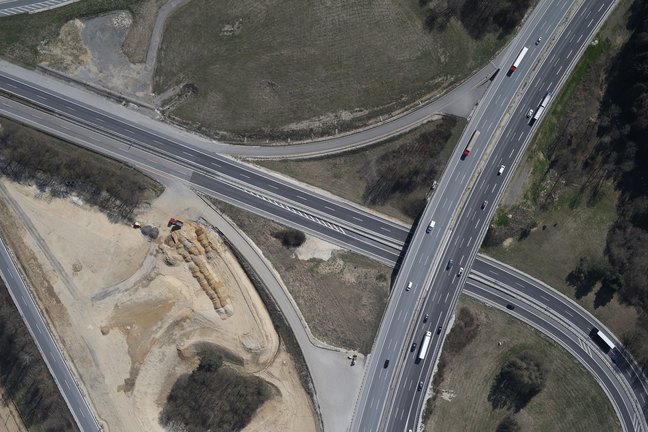
\includegraphics[width=0.45\textwidth]{L1234_rsz.png}
    \caption{\small Original Image}
    \label{fig:OriImg}
  }
  \quad
  \parbox{.475\linewidth}{
    \centering
    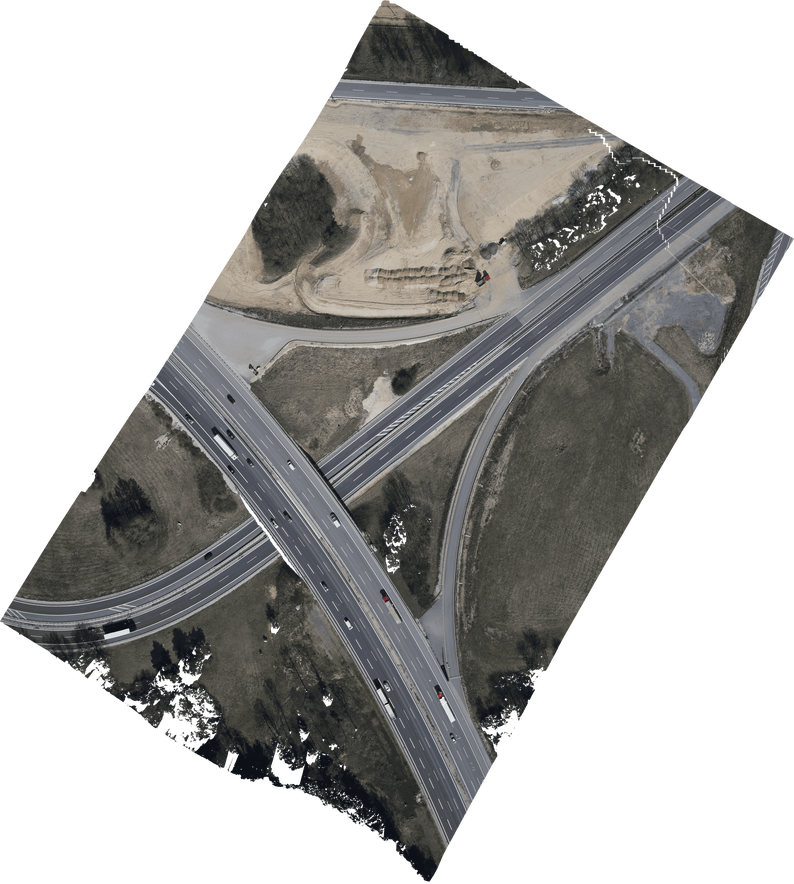
\includegraphics[width=0.45\textwidth]{OL1234_rsz.png}
    \caption{\small Orthorectified Image}
    \label{fig:OrthoImg}
  }
  \centering
  \parbox{.7\linewidth}{
    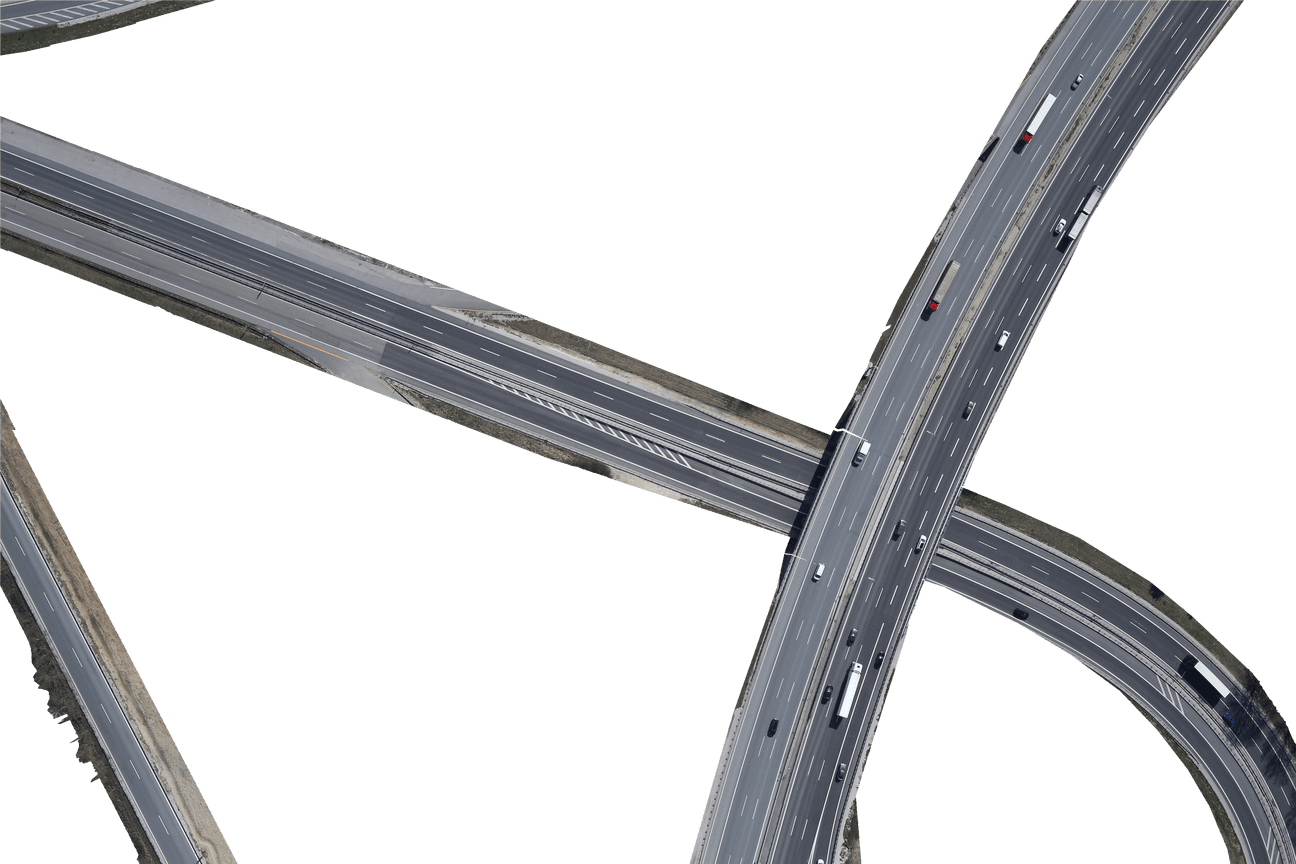
\includegraphics[width=0.7\textwidth]{ML1234_rsz.png}
    \caption{\small Masked Image}
    \label{fig:MaskedImg}
  }
\end{figure}

\clearpage
%%%%%%%%%%%%%%%%%%%%%%%%%%%%%%%%%%%%%%%%%%%%%%%%%%%%%%%%
\section{Preprocessing}
\label{sec:preprocessing}

In lane marking extraction step, the $\sigma$ value for Gaussian smoothing is set to be 1.8 % From HALCON Referenz: For the choice of the thresholds High and Low one has to keep in mind that the second directional derivative depends on the amplitude and width of the line as well as the choice of Sigma. Thus: you must set this value depending on the lane marking width?
to slightly suppress the noise in images.
The extracted lines of length less than 70 pixels are rejected % why
regarding the fact that a dashed lane-line is no longer than 6 meter which is correspondingly 87 pixels with GSD of 6.9 cm.
% http://www.mvtec.com/doc/halcon/11/en/lines_gauss.html
% https://www.dvr.de/download/publikationen-schriftenreihe-17.pdf

table:
simu.case1: noisy measurements and biased initial values of the unknowns

covering images, observations, unknowns, redundancies, 


%%%%%%%%%%%%%%%%%%%%%%%%%%%%%%%%%%%%%%%%%%%%%%%%%%%%%%%%
\section{Simulation}
\label{sec:simulation}
This section aims to verify the correctness of the derived LS model using simulation data. The used materials are as described in \cref{sec:Materials}. Only the measurements (the image coordinates of the extracted lines), the true and approximate values of the unknowns (the object coordinates of a line segment) in the non-linear LS model are simulated, as described in \cref{subsec:simudata}.

\cref{subsec:simuresult} aims to check if the iteration scheme converges to the correct solution given imperfect initial values of the unknowns. This subsection also presents the significant height differences between the approximate and the reconstructed line segments, indicating the necessity of refinement base on image triangulation.
%\cref{subsec:simuresult-2} checks, without the influences from camera parameters' quality, if the derived LS model is able to resist the simulated random errors contained in the measurements.

Note that the quality of camera parameters (EO., IO. and additional parameters) do not have influences in simulation since the simulated measurements are produced with the same set of camera parameters as the set used for 3D reconstruction.



\subsection{Simulation Data}
\label{subsec:simudata}

\paragraph{The true line segment in object space}
Firstly, the object coordinates of the endpoints of a 3D line segment are defined, with 136 meters length, locating on the road surface in the test area (German highway A9) with 3 to 7 aerial images coverage. By linear interpolating several points with 0.2 meter spaces (considering DSM grid of 0.2 meter) between the two endpoints, a 3D line segment in the form of a set of 3D points is generated. This 3D line segment serves as the ground truth in the experiments in \cref{sec:simulation}. 

\paragraph{The observed line segments in image spaces}
The observations in the LS model are simulated by back-projecting the true line segment into the covering images. Gaussian random noise $e\sim\mathcal{N}(0,0.5^2)$ is added in the observations for each LS adjustment, as line extraction process is of sub-pixel accuracy. The added noise is plotted in \cref{fig:noise}

\begin{figure}
  \centering
  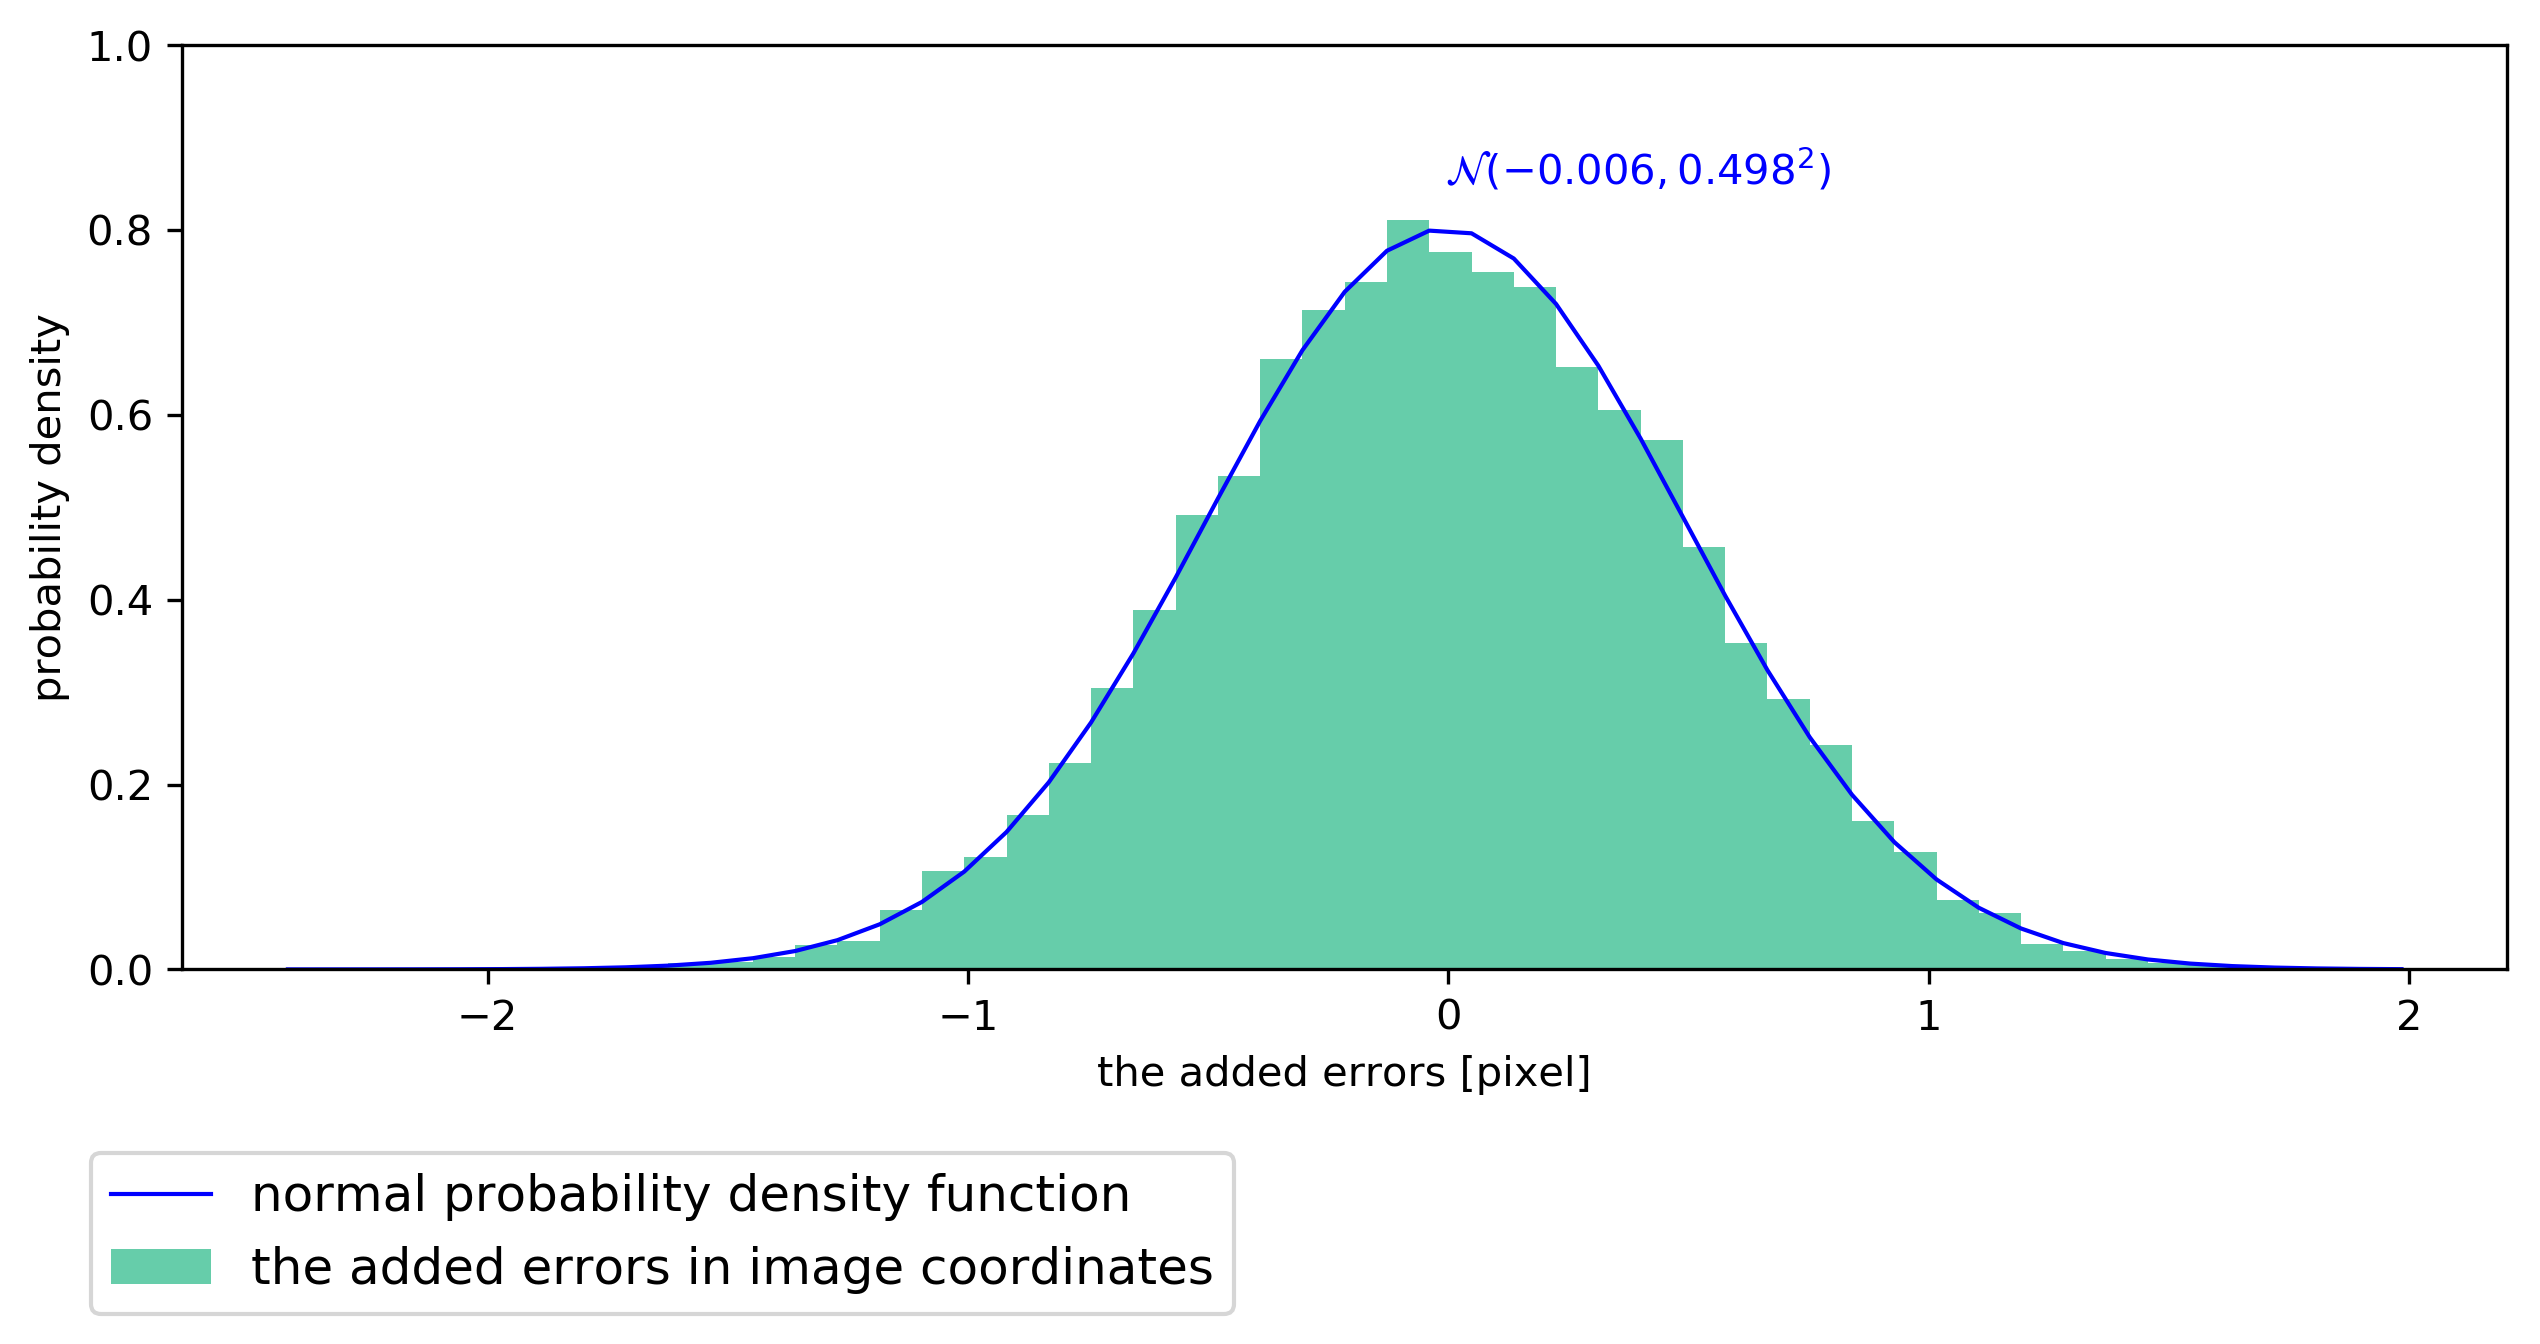
\includegraphics[width=0.8\textwidth]{Simu_errorhist_1.png}
  \caption{\small The added Gaussian random noise in the observations.}
  \label{fig:noise}
\end{figure}

\paragraph{The approximate line segment in object space}
The initial estimates for non-linear LS adjustment is generated by projecting the observed line segments in image space onto the DSM.

\clearpage

\subsection{Simulation Result}
\label{subsec:simuresult}

%%% analysis on the unknowns:
\cref{fig:Simu3D_2} shows the reconstructed and the true line segments in UTM coordinate system (in Zone 32N). The distances from the reconstructed line nodes to the true line segment are collected, resulting in sample size of $18$. The sample mean is $0.008$ [meter] and the sample variance is $0.101$ [meter]. % This sampling procedure is assumed to be independent and random.%??? (t test assumptions)

For such small sample size data, a two-tailed t-test is adopted to test if the population mean significantly not equals zero, i.e. \textbf{if the reconstructed line segments are significantly far from the true line segments}. Null hypothesis ($H_0$) and (two-tailed) alternative hypothesis ($H_A$) are stated as:
\begin{equation*}
\begin{split}
H_0: \mu=0\\
H_A: \mu\neq0
\end{split}
\end{equation*}

A significance level $\alpha=0.05$ is selected, with degree of freedom being $18-1=17$, the two-tailed t-table value $T_{(0.975,17)}$ is
\begin{equation*}
T_{(0.975,17)}=2.110
\end{equation*}
which leads to the decision rule: if test statistic $T_{obs}$ is less than $-T_{(0.975,17)}=-2.110$ or greater than $T_{(0.975,17)}=2.110$, reject the null hypothesis.

With the sample mean $\overline{x}=0.008$,
the proposed population mean $\mu_0=0$,
the sample standard deviation $\sigma=0.101$,
and sample size $n=18$, the test statistic for One Sample T Test has the calculated value:
\begin{equation*}
T_{obs} = \frac{\overline{x}-\mu_0}{\sigma/\sqrt{n}}=\frac{0.008-0}{0.101/\sqrt{18}}\approx0.34
\end{equation*}
which is neither less than $-T_{(0.975,17)}=-2.110$ nor greater than $T_{(0.975,8)}=2.110$, i.e. not in the rejection region. As a result, we fail to reject the null hypothesis. In other words, \textbf{we are not able to claim that the reconstructed line is significantly far away from the true line}. This indicates that \textbf{the derived non-linear LS adjustment model for 3D reconstruction is correct}.

\cref{fig:Simu3D_1} shows the reconstructed line segments and the DSM profile which serves as the initial approximation for non-linear LS adjustment, in UTM coordinate system (in Zone 32N). The maximum distance between them is 1.97 meter, mainly in Z-direction. This tells that \textbf{the reconstruction model is at least able to refine the initial approximation with 2 meters bias in Z-direction}.

\begin{figure}
  \centering
  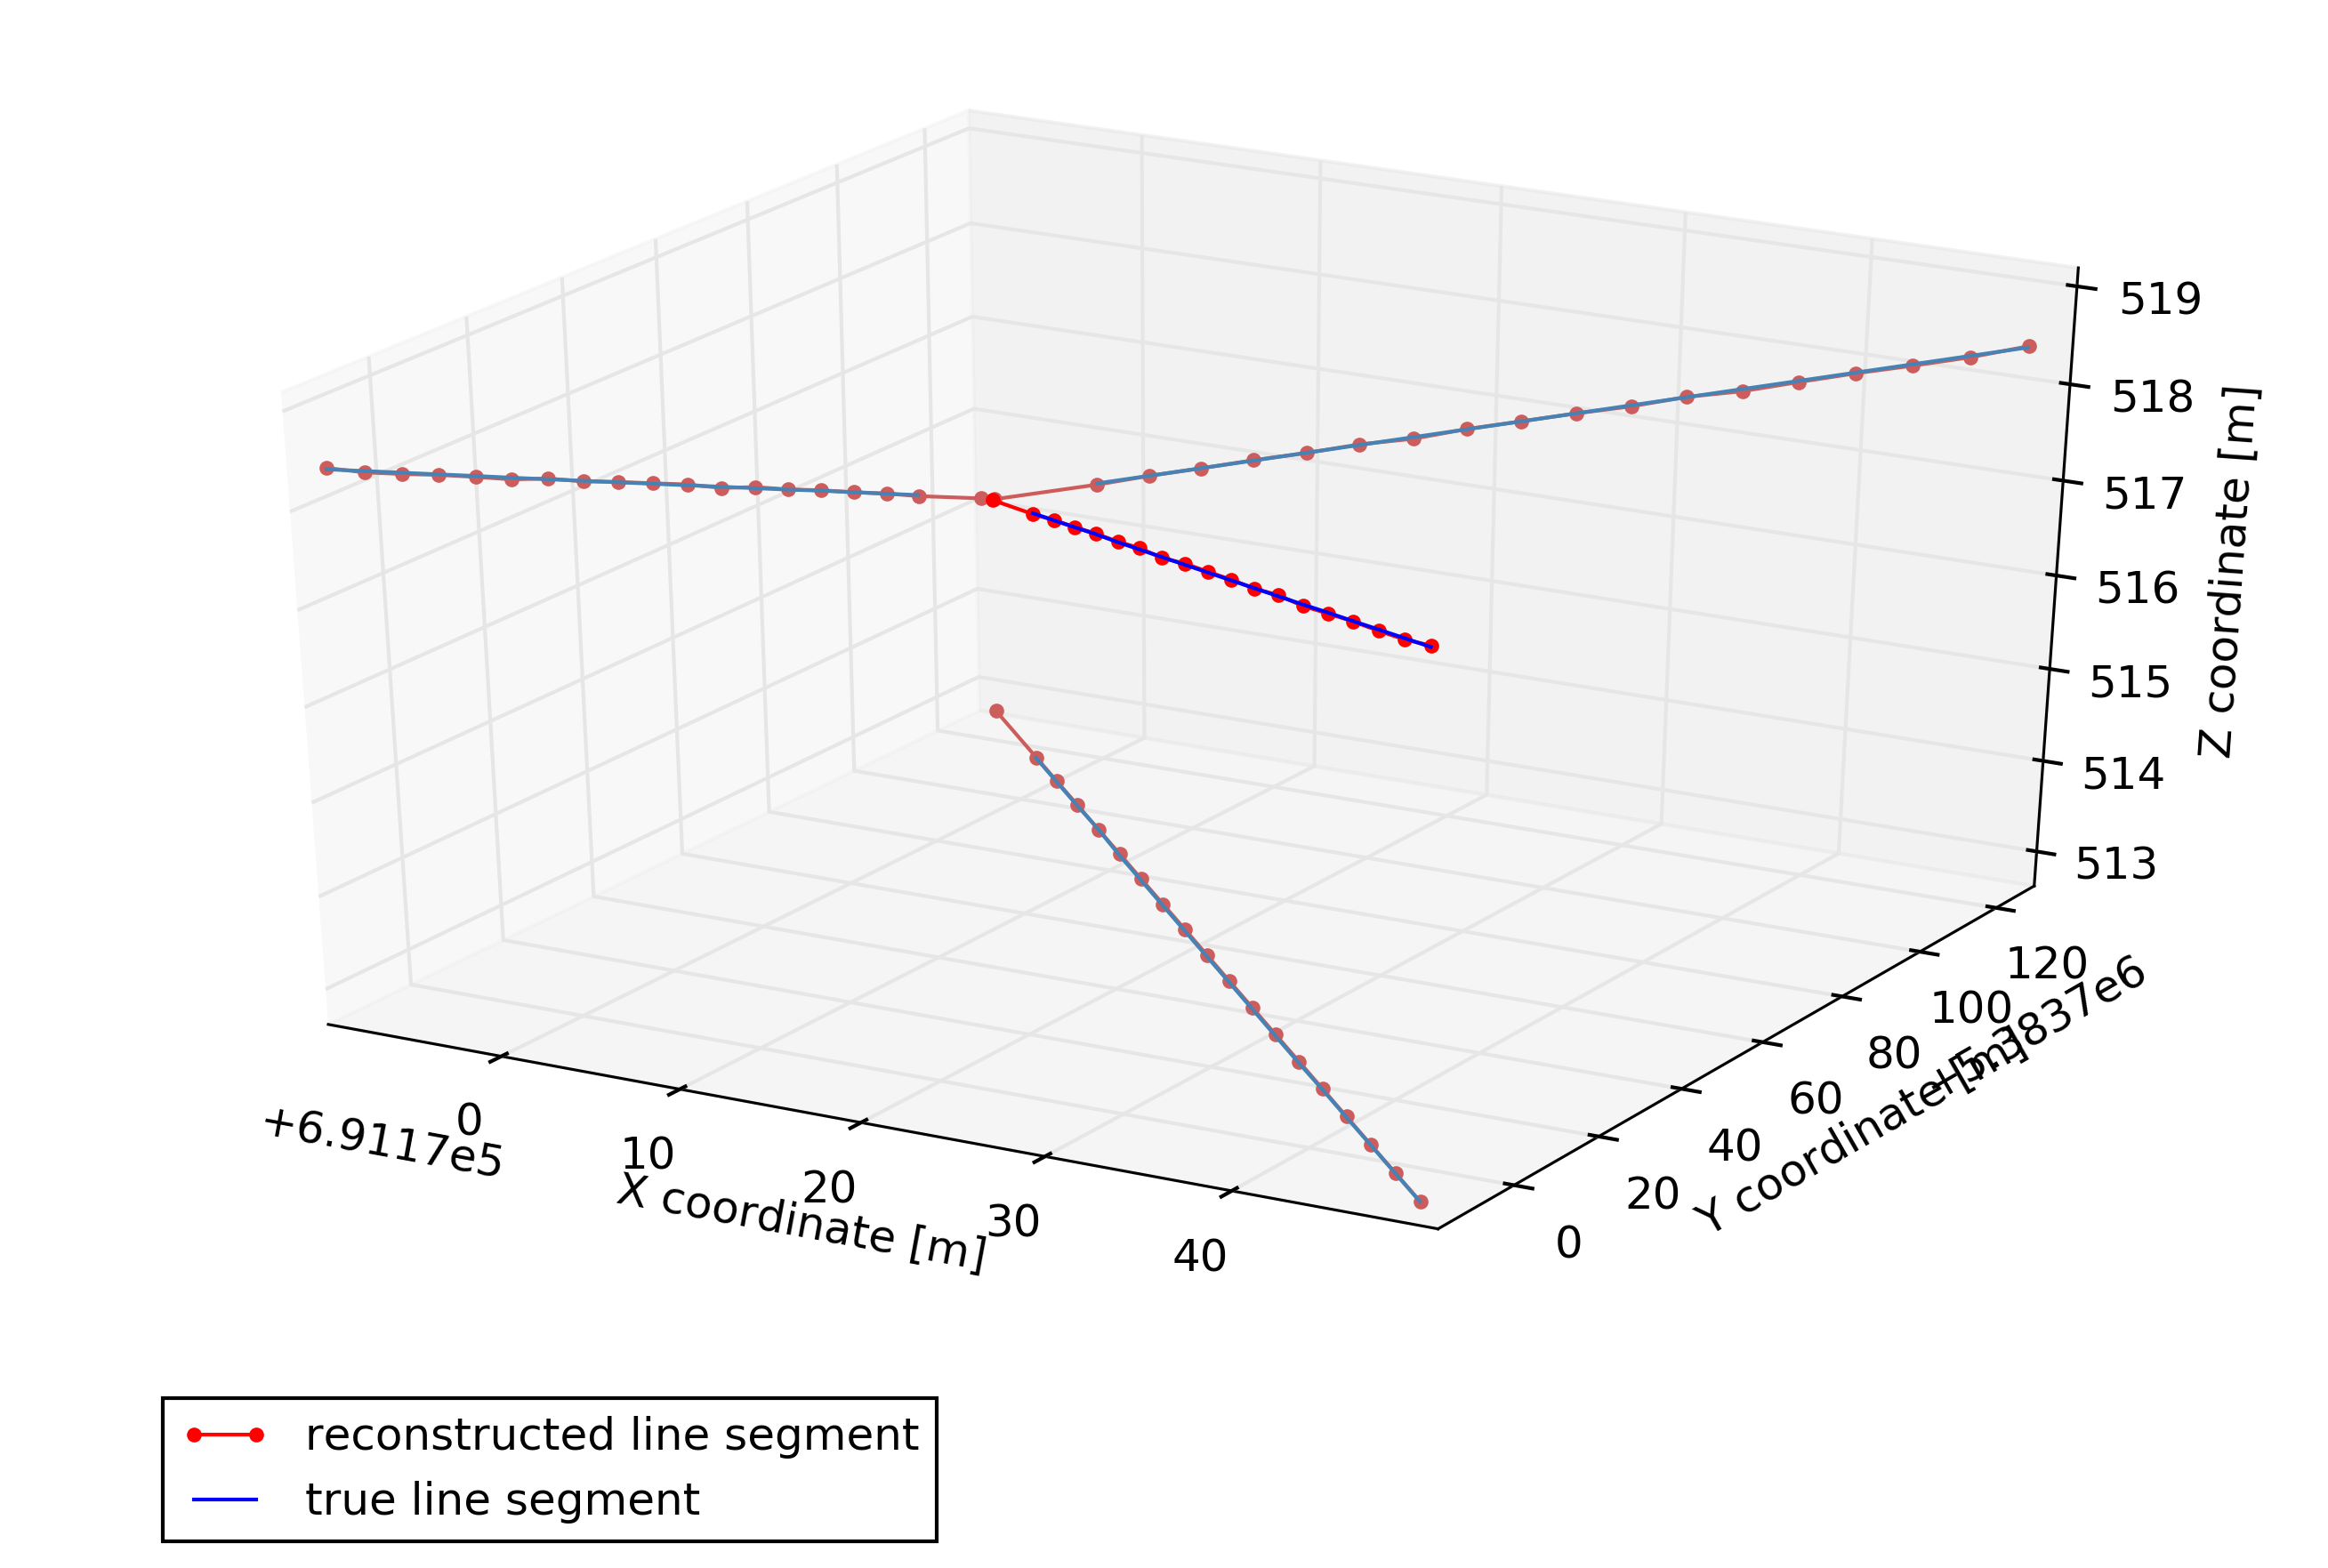
\includegraphics[width=\textwidth]{Simu_3D_2.png} %%% 換,字重疊。
  \caption{\small The reconstructed line segments and the true line segments in UTM coordinate system (in Zone 32N).}
  \label{fig:Simu3D_2}
  \vspace{1cm}
  \centering
  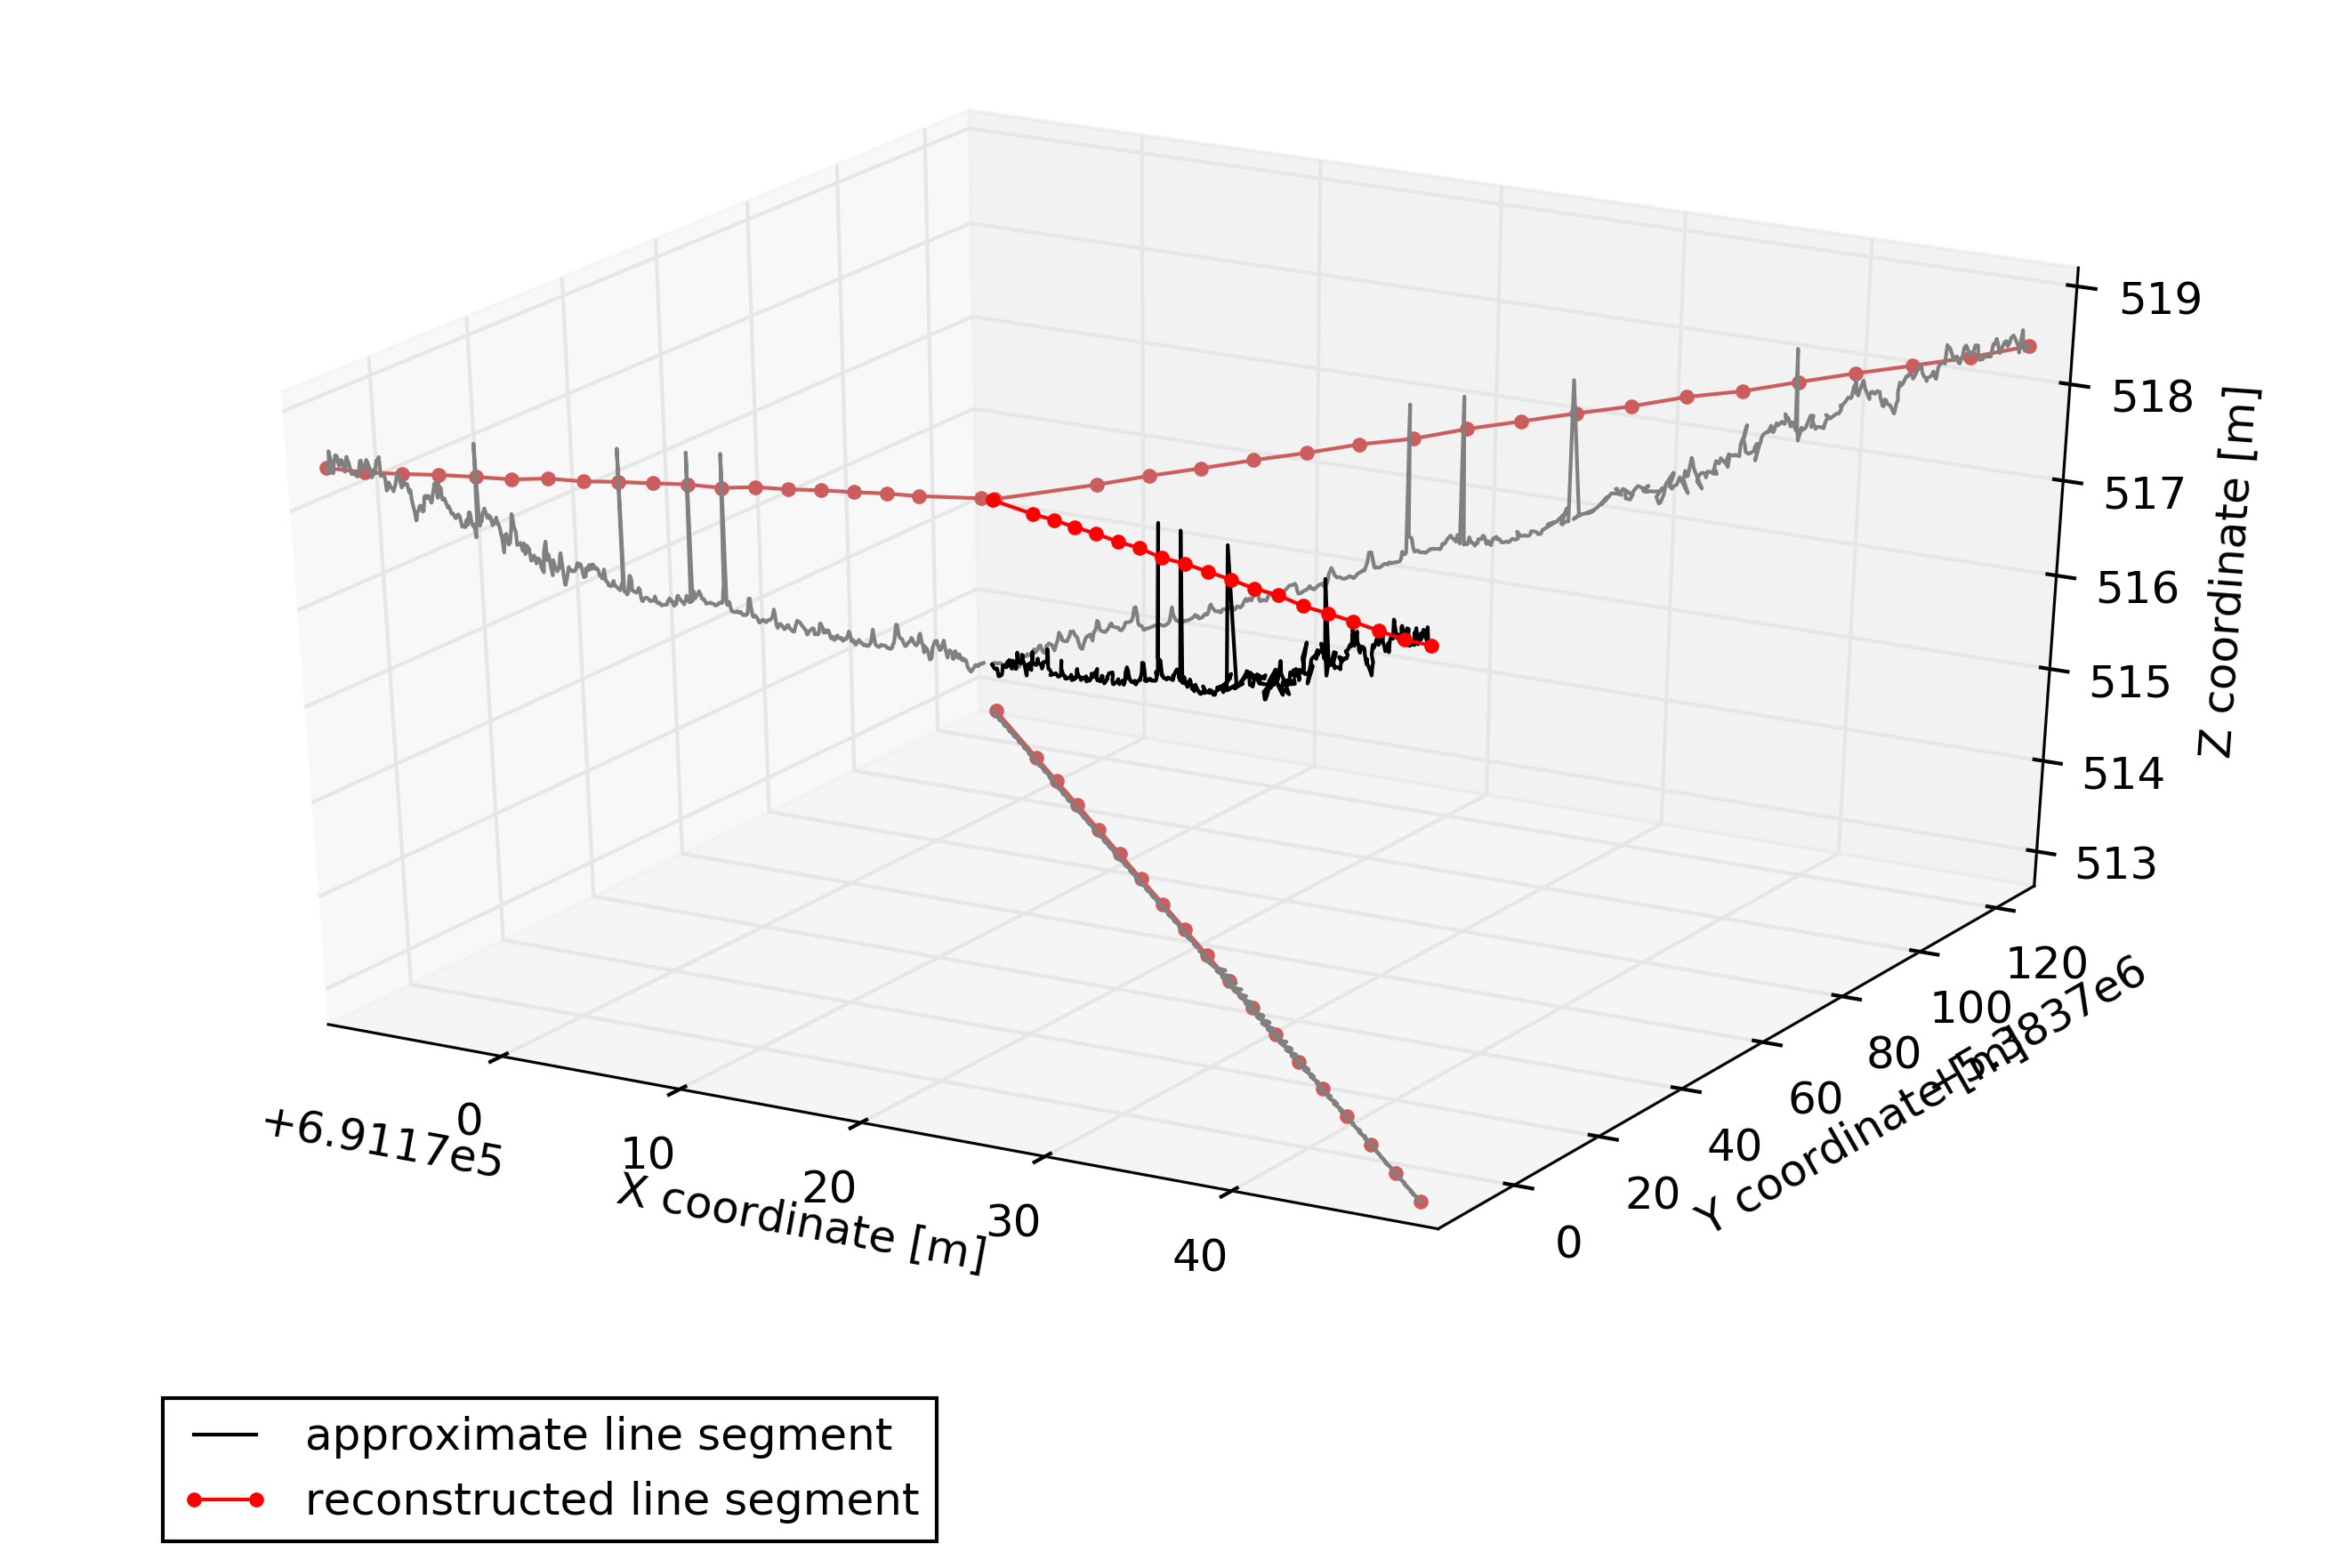
\includegraphics[width=\textwidth]{Simu_3D_1.png}
  \caption{\small The reconstructed line segments and the unrefined DSM profile in UTM coordinate system (in Zone 32N).}
  \label{fig:Simu3D_1}
\end{figure}

\clearpage




%The distances from the reconstructed line segment to the DSM profile are plotted into histogram in \cref{fig:SimuHist_1}. They are collected along the reconstructed line segments with 0.2 meter spacing (considering the DSM grid of 0.2 meter), resulting in sample size of $381$. The sample mean is $-0.029$ [meter] and the sample variance is $0.083$ [meter]. % This sampling procedure is assumed to be independent and random.%??? and normal distributed (Z test assumptions)

%In order to know \textbf{if the mean distance from the reconstructed line segments to the DSM profile is significantly non-zero}, a two-tailed Z-test is adopted for such big sample size cases. Null hypothesis ($H_0$) and (two-tailed) alternative hypothesis ($H_A$) are stated as:
%\begin{equation*}
%\begin{split}
%H_0: \mu=0\\
%H_A: \mu\neq0
%\end{split}
%\end{equation*}

%A significance level $\alpha=0.05$ is selected, which is $0.025$ on each tail of the population, i.e. the area in body is $0.975$ out of 100\%. The corresponding z-score is:
%\begin{equation*}
%Z_{0.975}=1.96
%\end{equation*}
%which leads to the decision rule: if $Z_{obs}$ is less than $-1.96$ or greater than $1.96$, reject the null hypothesis.

%With the sample mean $\overline{x}=-0.029$,
%the proposed population mean $\mu_0=0$,
%the sample standard deviation $\sigma=0.083$,
%and sample size $n=381$, the test statistic for a One Sample Z Test has a calculated value:
%\begin{equation*}
%Z_{obs} = \frac{\overline{x}-\mu_0}{\sigma/\sqrt{n}}=\frac{-0.029-0}{0.083/\sqrt{381}}\approx-6.82
%\end{equation*}

%As the test statistic $Z_{obs}\approx-6.82$ is less than $-Z_{0.975}=-1.96$, i.e. in the rejection region, the null hypothesis is rejected. In other words, \textbf{with 95\% confidence we can claim that the mean distance from the reconstructed line segment to the DSM profile is significantly non-zero}. This phenomenon is as expected, as mentioned in sec:DSM???. 



\cref{fig:SimuImgNum} gives the information on the amount of covering images, the redundancies and the height value of the reconstructed nodes, of each segment. Note that in each segment, LS adjustment is processed independently.

\begin{figure}
  \centering
  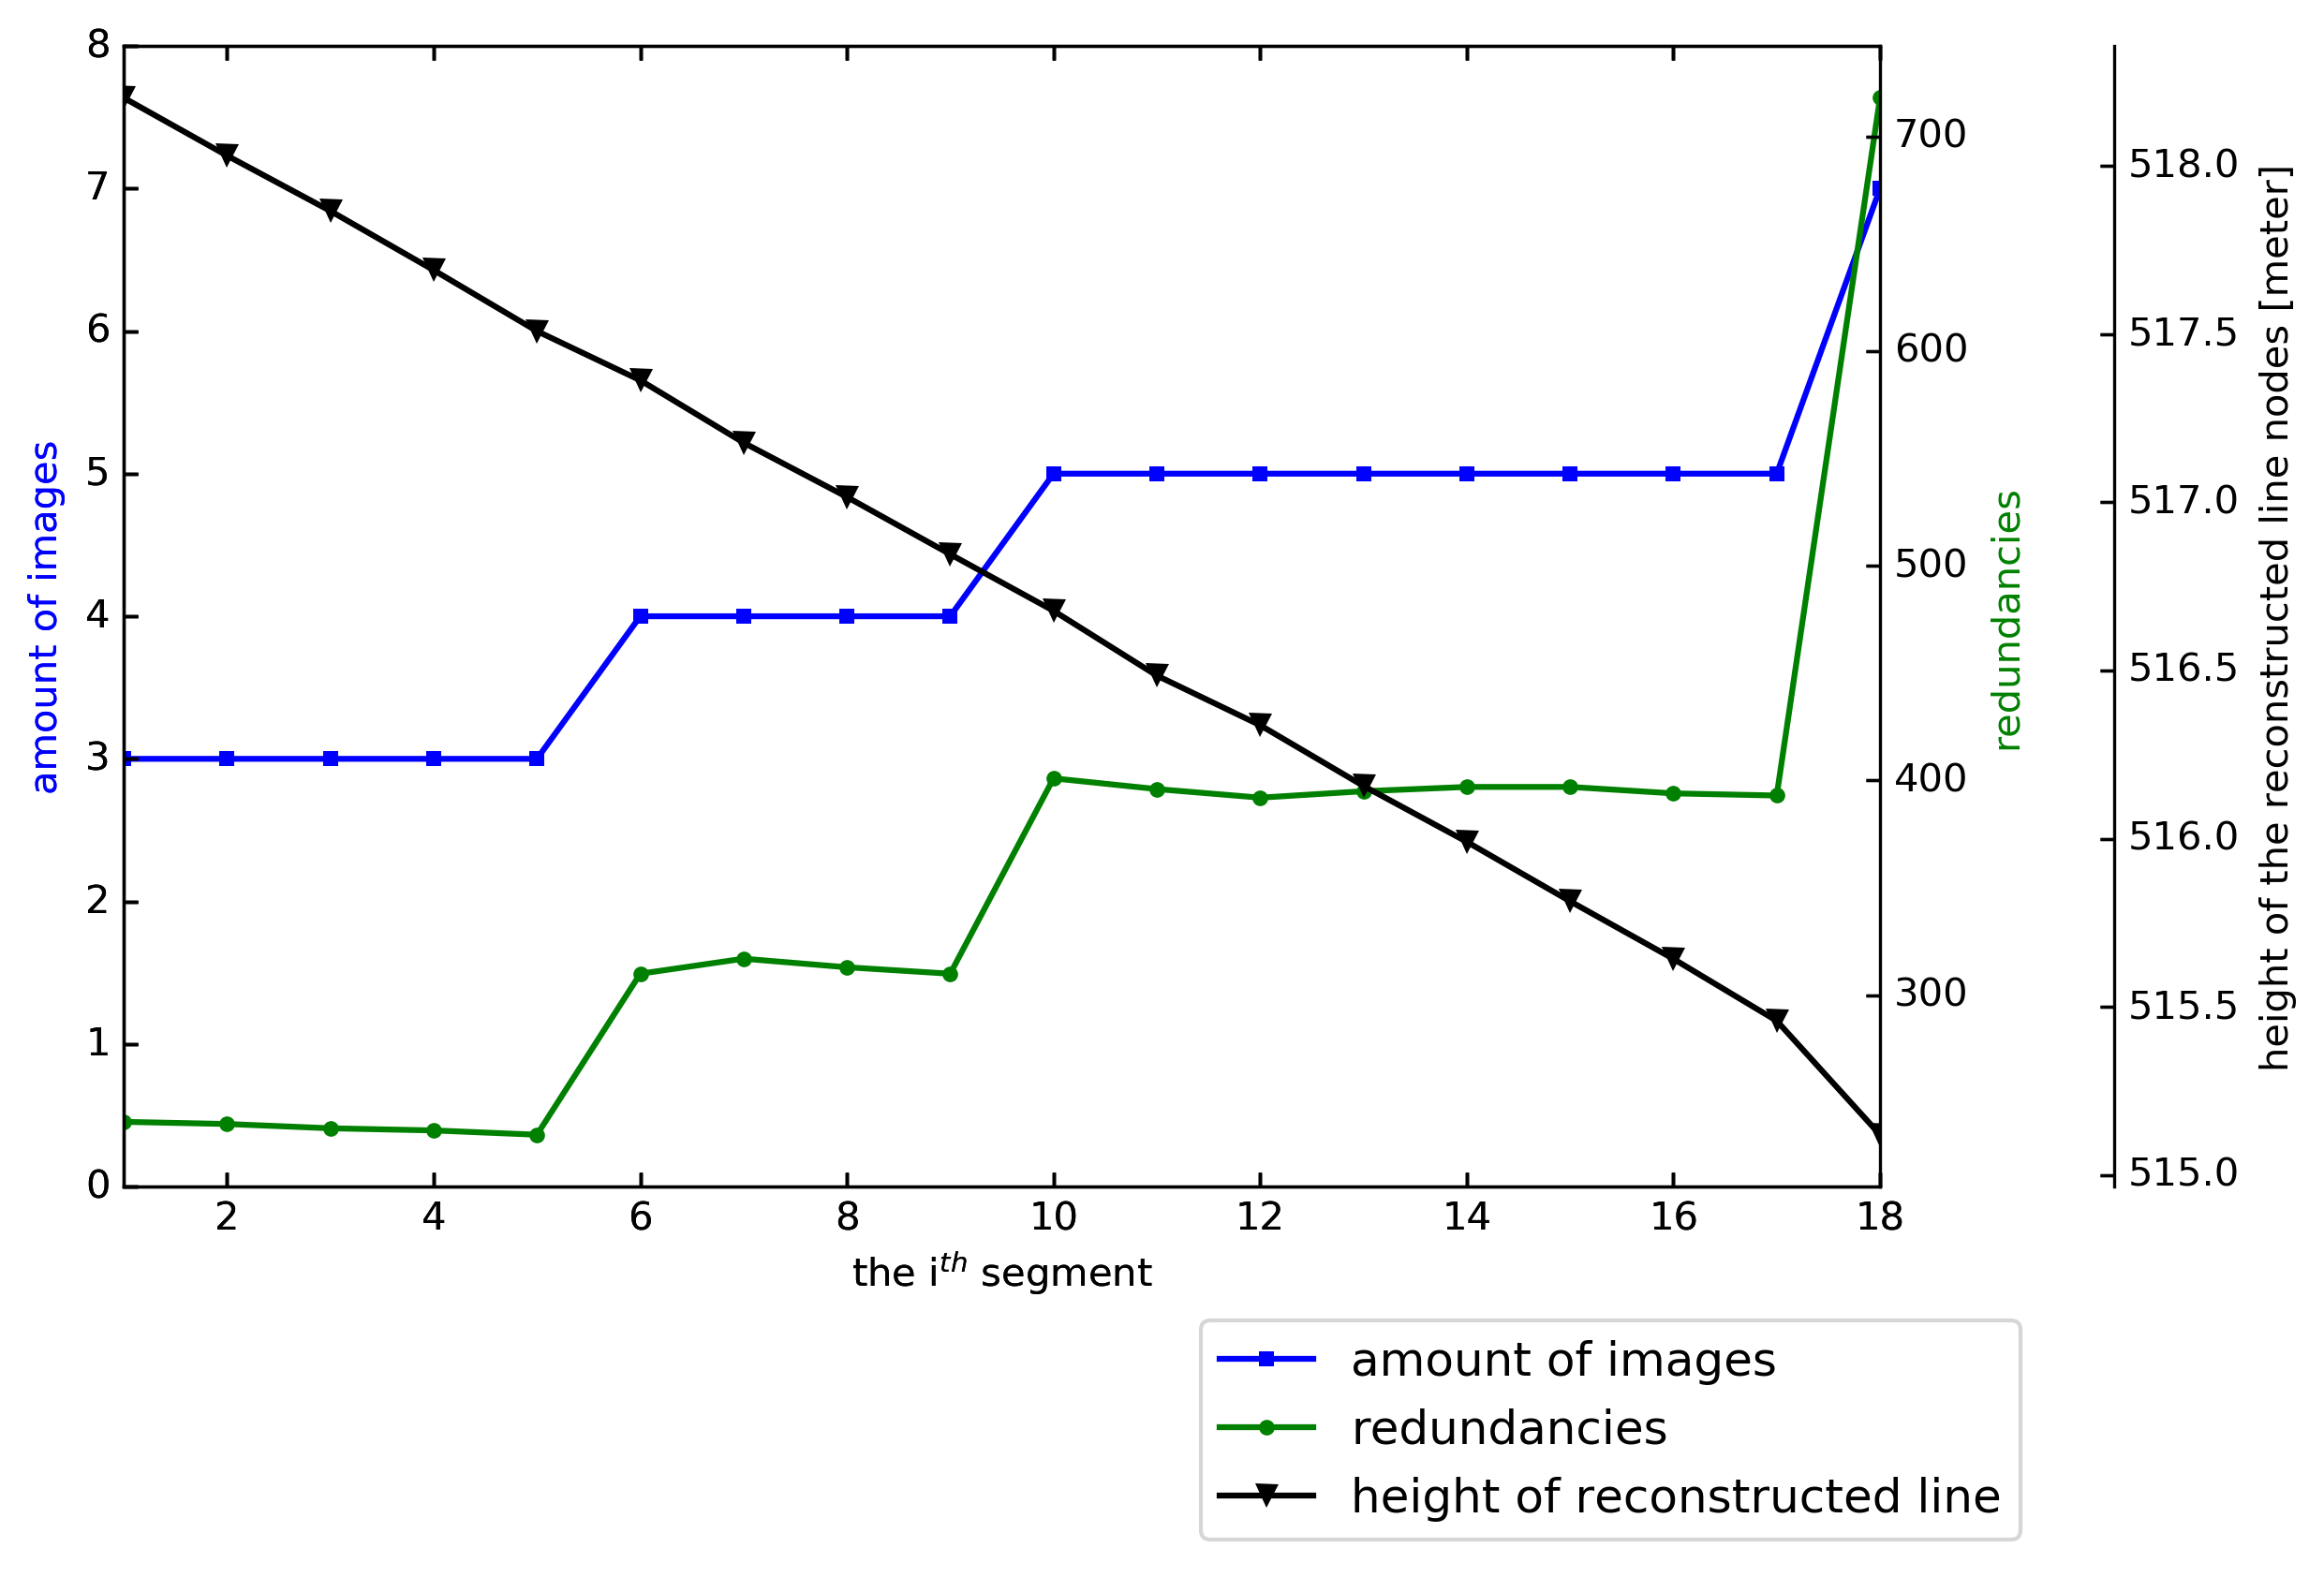
\includegraphics[width=\textwidth]{Simu_ImgNum.png}
  \caption{\small XXX.}
  \label{fig:SimuImgNum}
\end{figure}

%%% analysis on measurements:
\cref{fig:SimuError} shows the mean and variance of the added random Gaussian noise and the adjusted residuals of each segment. This two samples are compared by applying a two-tailed two-sample T-test. Null hypothesis and alternative hypothesis ($H_A$) are stated as:
\begin{equation*}
\begin{split}
H_0: \mu_1-\mu_2=0\\
H_A: \mu1-\mu_2\neq0
\end{split}
\end{equation*}

With significance level $\alpha=0.05$ and degree of freedom $\approx300$, the t-score is 
\begin{equation*}
T_{0.95,300}=1.968
\end{equation*}

As shown in \cref{fig:SimuTtest}, all the test statistics $T_{obs}$ of each segment are not less than $-T_{0.95,300}=-1.968$ or greater than $T_{0.95,300}=1.968$, i.e. not in the rejection region, the null hypothesis could not be rejected. In other words, 


%The redundancies increase with more covering images.
%The posterior standard deviation
%\begin{equation*}
%\hat{\sigma}_0=\sqrt{\dfrac{\sum\hat{e}^\mathsf{T}\hat{e}}{redundancy}}
%\end{equation*}
%reflects the measurement quality.
%posterior standard deviation appears to have no obvious correlation with the amount of images.  Unless the included measurements





\begin{figure}
  \centering
  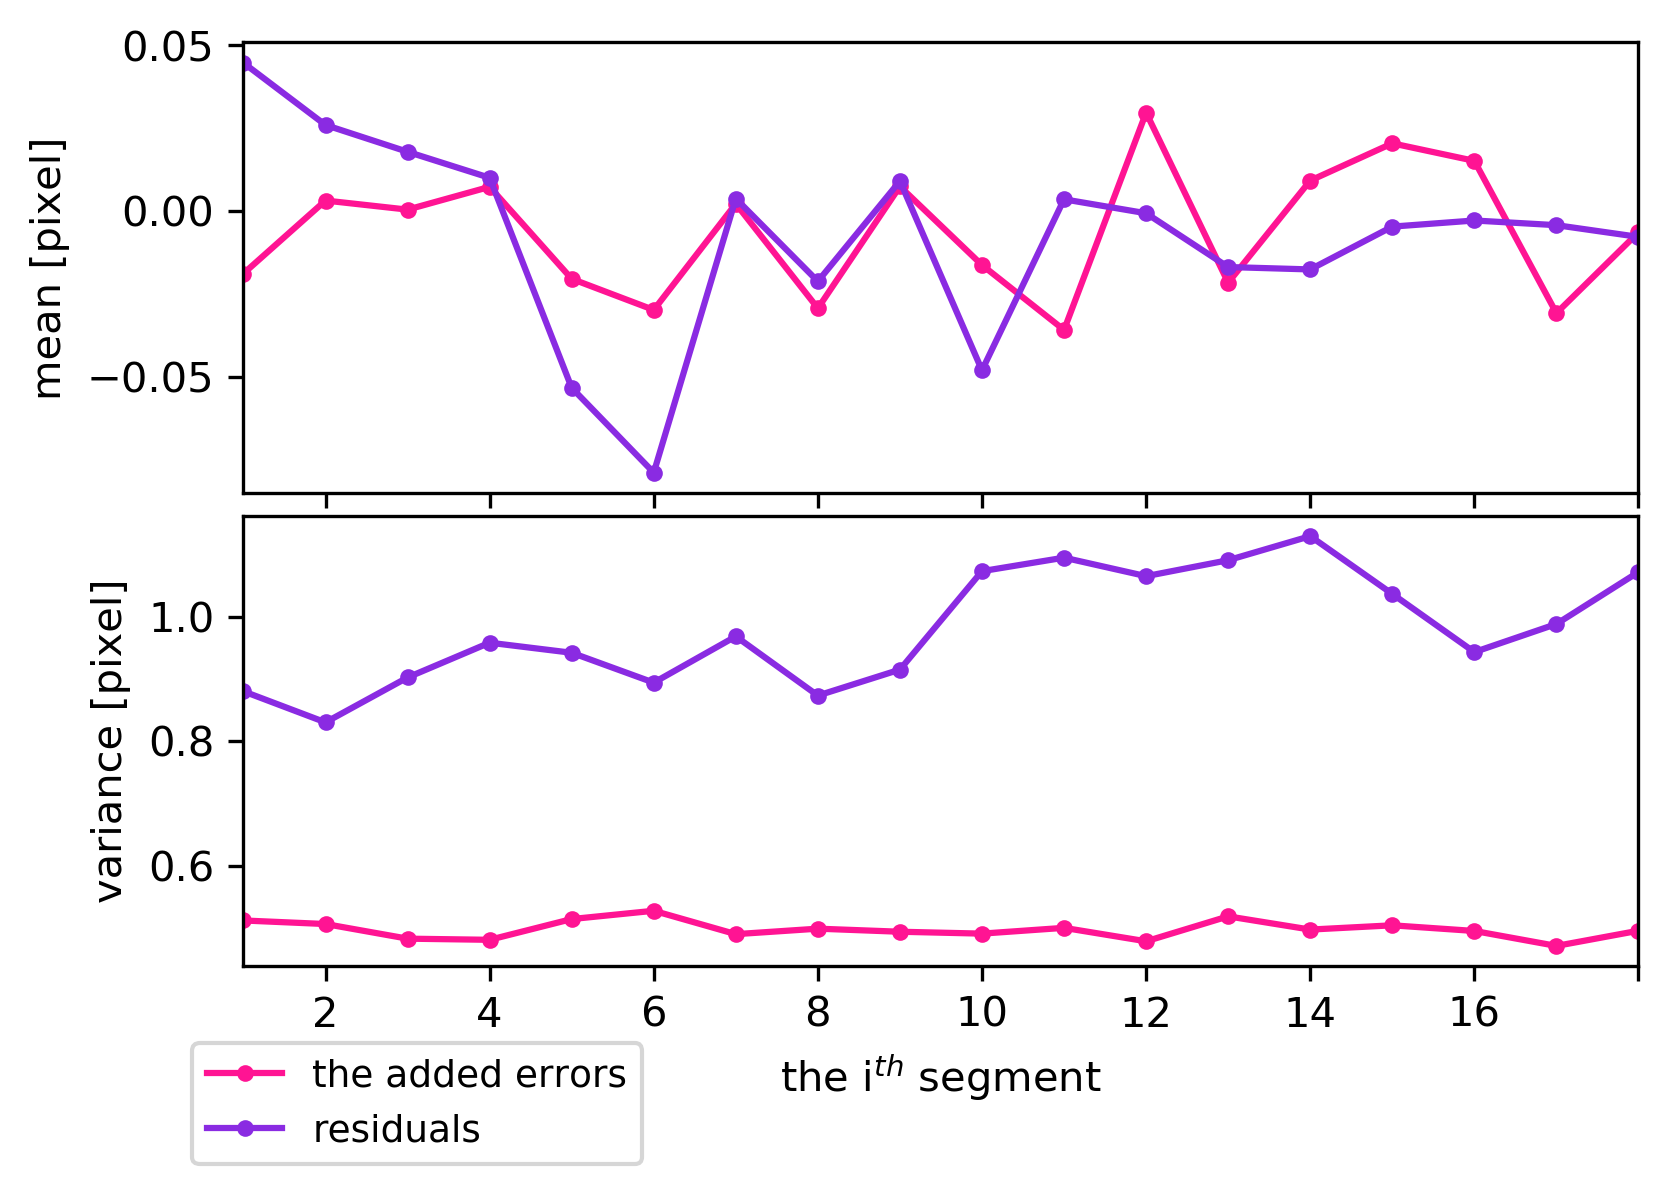
\includegraphics[width=0.95\textwidth]{Simu_error_1.png}
  \caption{\small The relation between the added random Gaussian noise and the adjusted residuals.}
  \label{fig:SimuError}
  \vspace{1cm}
  \centering
  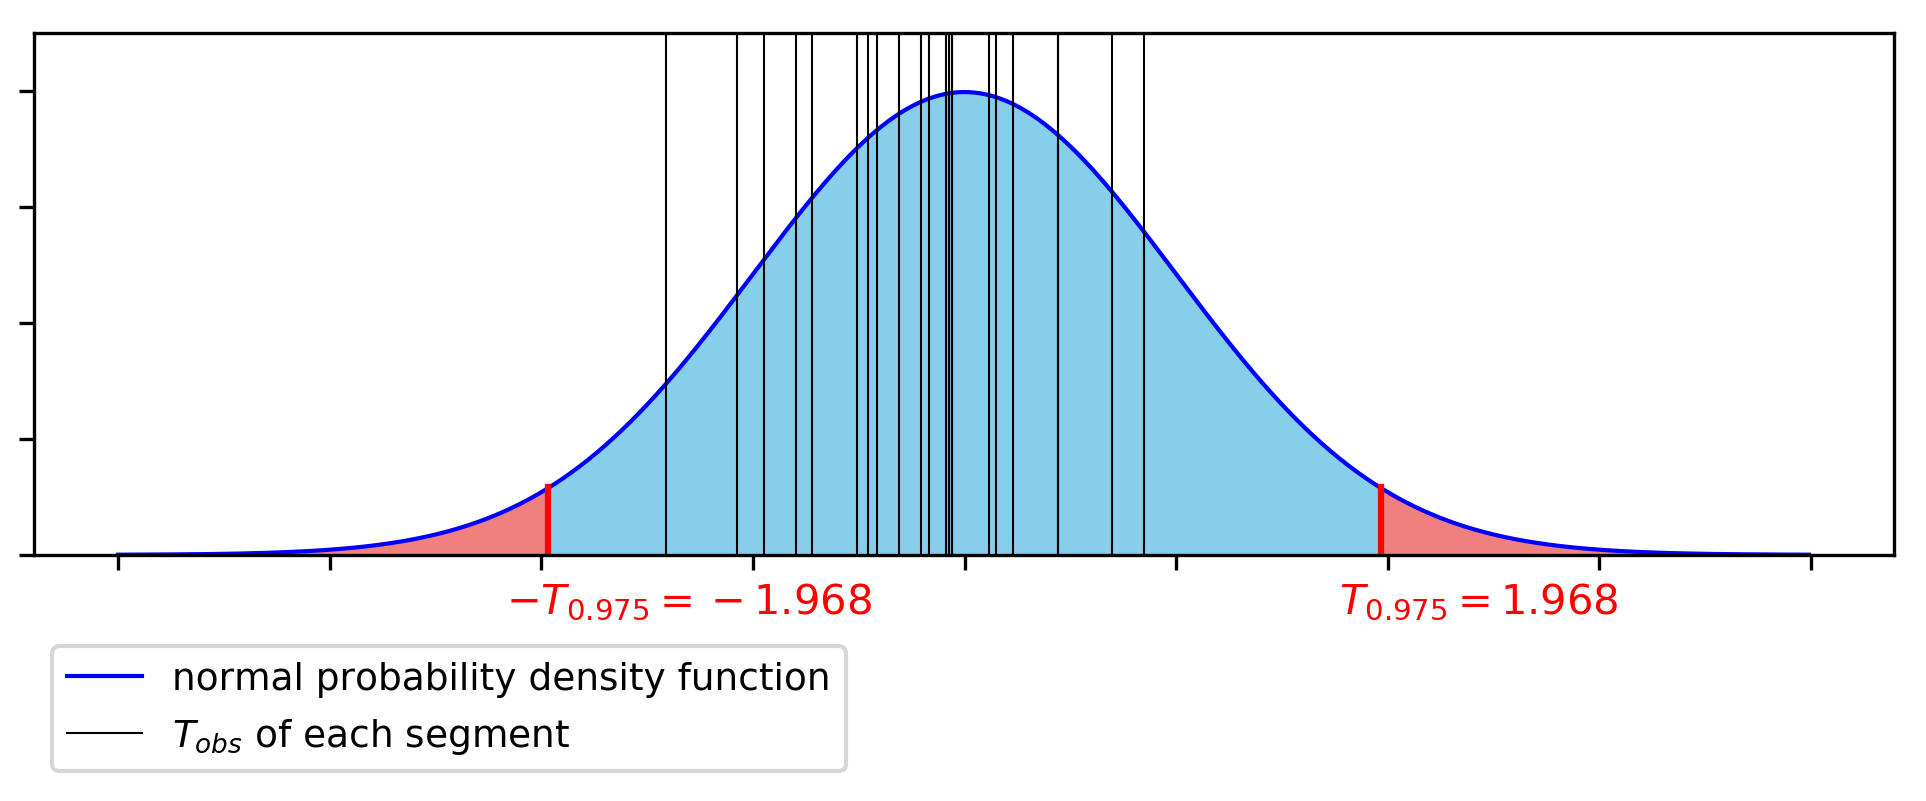
\includegraphics[width=\textwidth]{Simu_Ttest.png}
  \caption{\small The red area under the probability density function is the rejection region, which is 5\%. Since non of the $T_{obs}$ falls in the rejection region, the null hypothesis could not be rejected, i.e. we fail to claim that the adjusted residuals are different from the added random noise.}
  \label{fig:SimuTtest}
\end{figure}

\clearpage


From \cref{fig:SimuSigmaxx} it can be seen that the estimated parameters generally have smaller priori variance values (in horizontal direction) $\sqrt{\sigma_{\hat{X}}^2+\hat{\sigma}_{\hat{Y}}^2}$ and (in vertical direction) $\sigma_{\hat{Z}}$ with the increase of covering images. Whereas larger deviations from the trend are contained in vertical direction. \textbf{By increasing the configuration strength, i.e. increasing the amount of covering images with different orientations, the precision of the estimated parameters can be improved}.

Besides, the priori variance of the estimated parameters is smaller in vertical direction $\sigma_{\hat{Z}}$ than in horizontal direction $\sqrt{\sigma_{\hat{X}}^2+\hat{\sigma}_{\hat{Y}}^2}$. This tells that \textbf{the reconstructed nodes have higher precision in vertical direction}. [reason? sec 3.1]


\begin{figure}
  \centering
  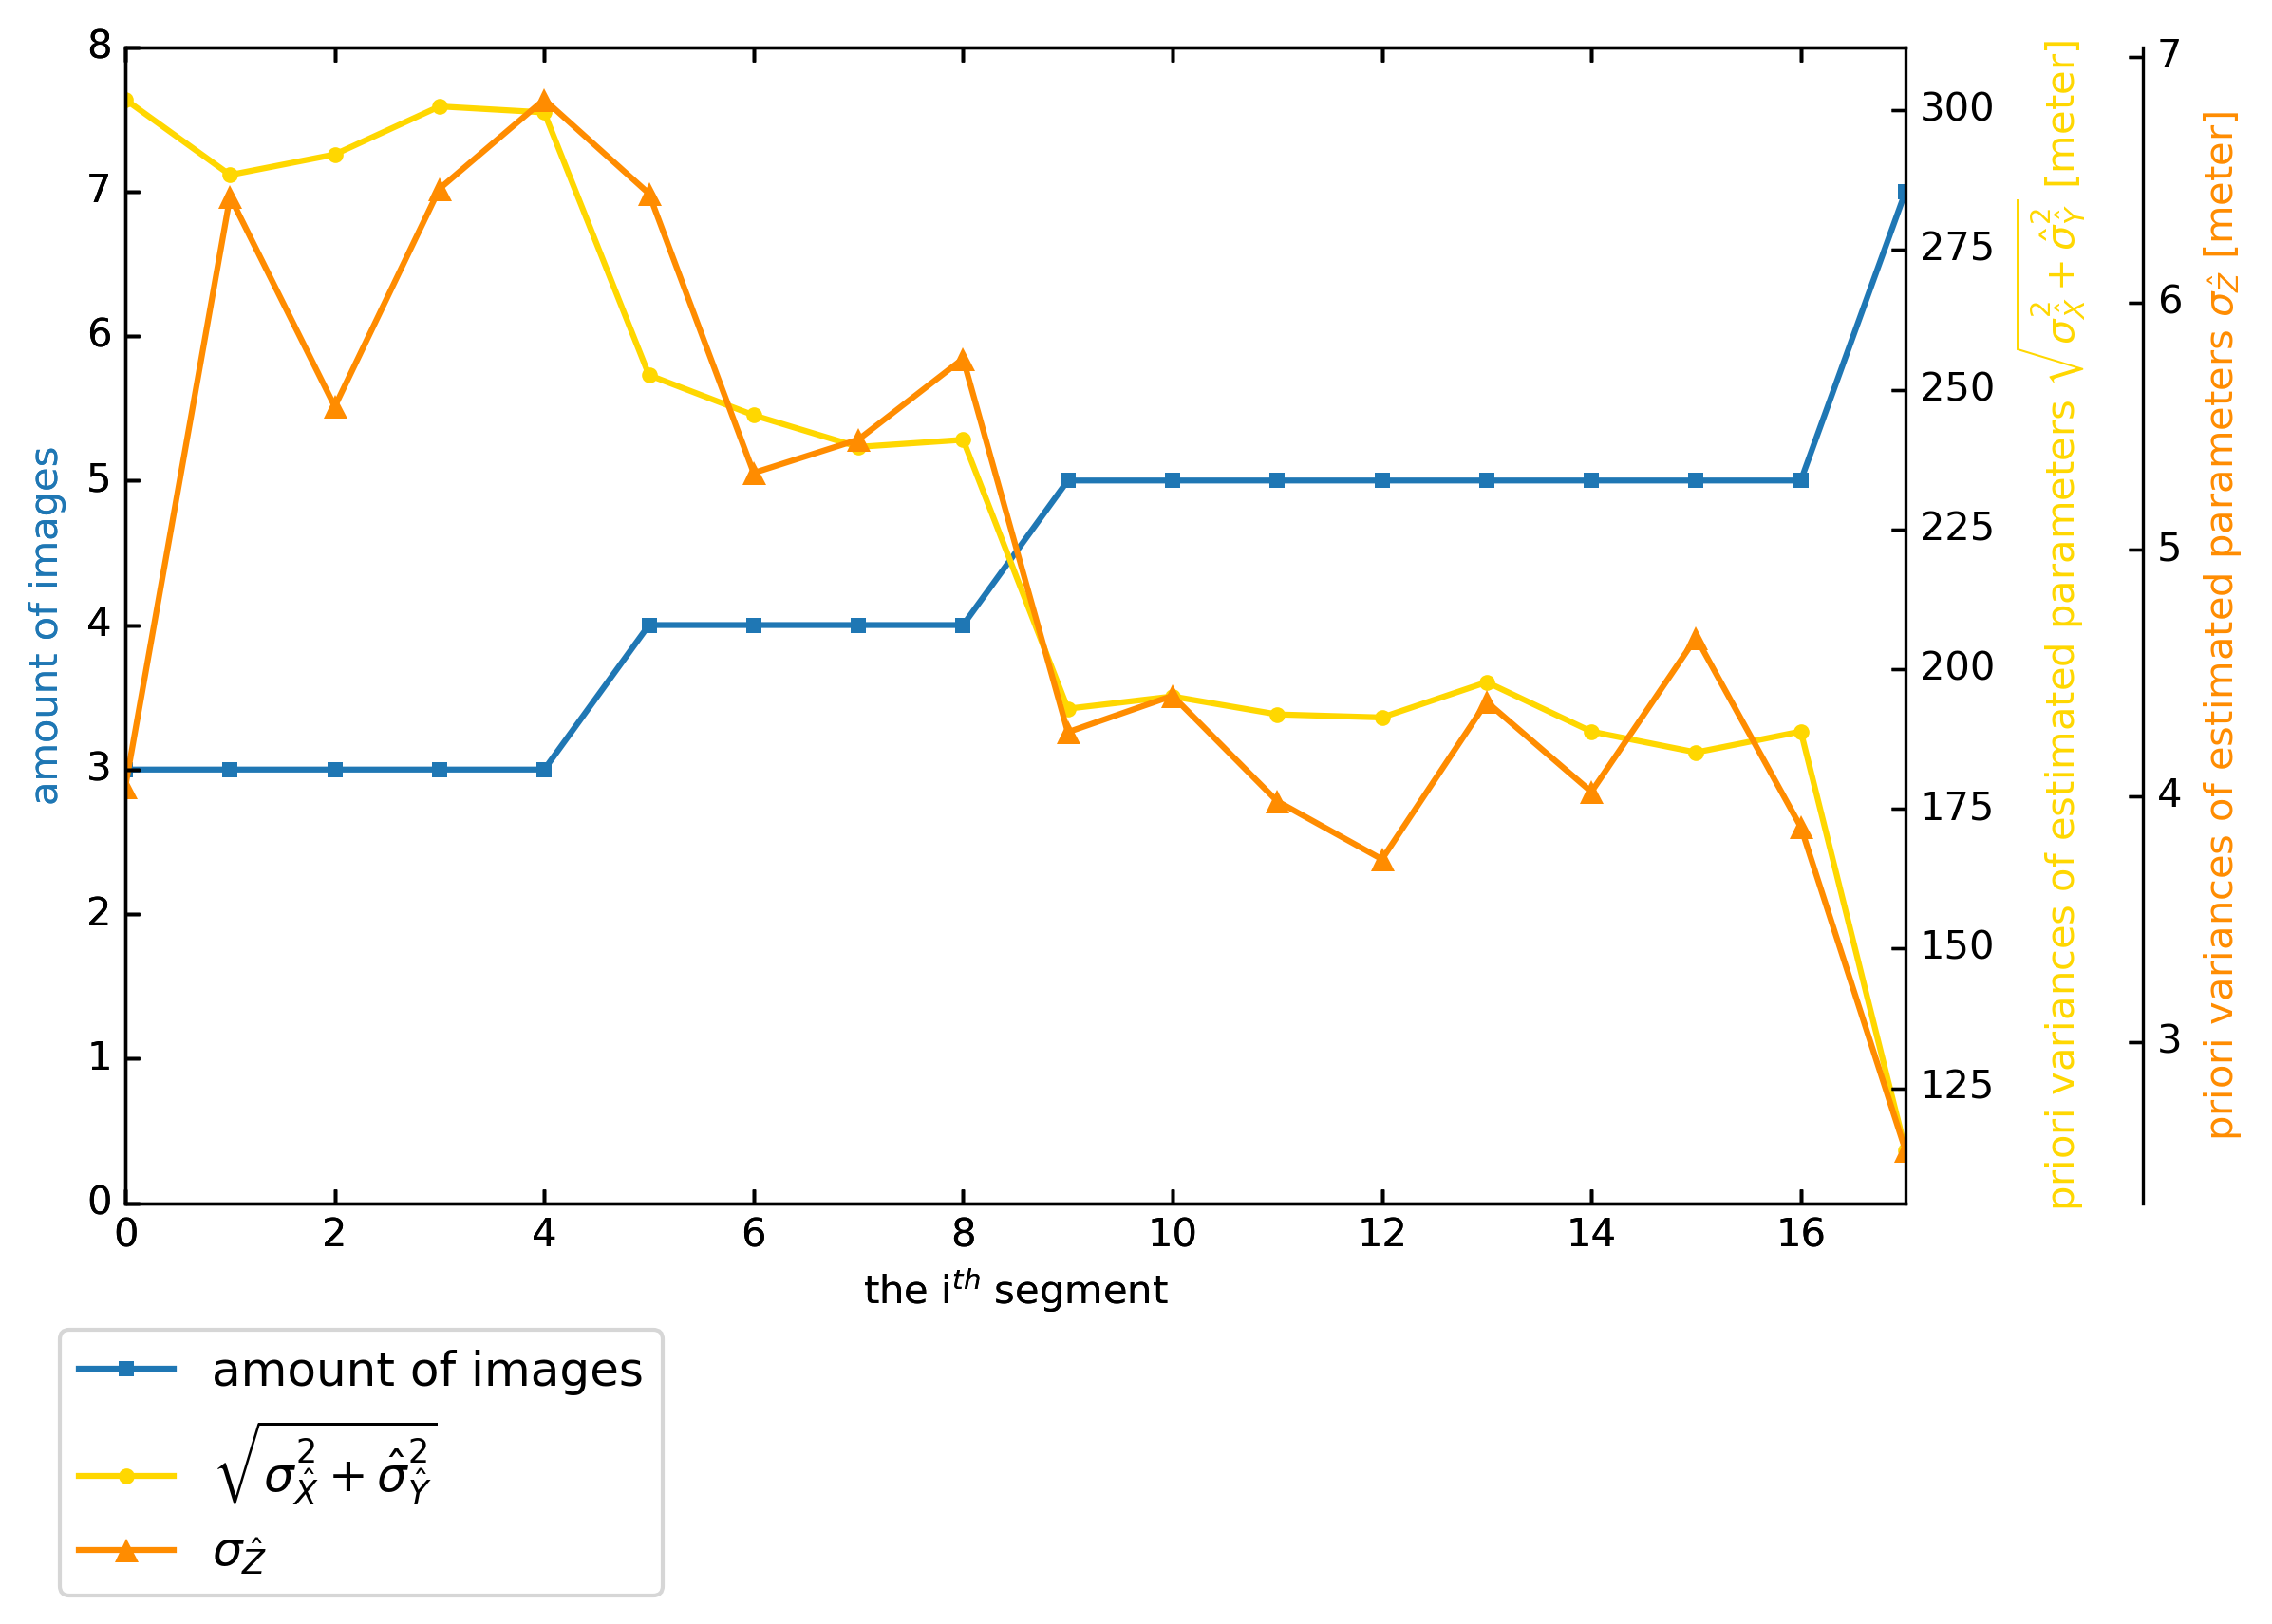
\includegraphics[width=0.95\textwidth]{Simu_XY_Z.png}
  \caption{\small The relation between the variances of the estimated parameters and the amount of images.}
  \label{fig:SimuSigmaxx}
\end{figure}

%%%%%%%%%%%%%%%%%%%%%%%%%%%%%%%%%%%%%%%%%%%%%%%%%%%%%%%%
\section{True Data}
\label{sec:truedata}

table:
%case1: Dashed Lane marking
case2: Continuous Lane marking%, two strips, multiple stereo pairs
%case3: Continuous Lane marking, two strips, two stereo pairs
%case4: Continuous Lane marking, two strips, one stereo pair
%case5: Continuous Lane marking, one strip

covering images, observations, unknowns, redundancies, 



%\subsection{True Data Result: case 1 -Dashed Lane Marking}
%\label{subsec:trueresult-1}


\subsection{True Data Result: case2 -Continuous Lane Marking}
\label{subsec:trueresult-2}

A continuous lane marking of ??? meters length is reconstructed. \cref{fig:Test3D_1} shows the reconstructed line segments and the DSM profile in UTM coordinate system (in Zone 32N). The distances from the reconstructed line segment to the DSM profile are plotted into histogram in \cref{fig:TestHist_1}. They are collected along the reconstructed line segments with 0.2 meter spacing (considering the DSM grid of 0.2 meter), resulting in sample size of $1256$. The sample mean is $-0.180$ [meter] and the sample standard deviation is $0.174$ [meter]. %This sampling procedure is assumed to be independent and random.%??? and normal distributed (Z test assumptions)

Assuming DSM height profile being significantly lower than the reconstructed line segments for more than $17$??? centimeters, a lower-tailed Z-test is adopted. Null hypothesis ($H_0$) and (one-tailed) alternative hypothesis ($H_A$) are stated as:
\begin{equation*}
\begin{split}
H_0: \mu\geq-0.170\\
H_A: \mu<-0.170
\end{split}
\end{equation*}

A significance level $\alpha=0.05$ is selected, i.e. the area in body is $0.950$ out of 100\%. The corresponding z-score is:
\begin{equation*}
Z_{0.950}=1.64
\end{equation*}
leads to the decision rule: if $Z_{obs}$ is less than $-1.64$, reject the null hypothesis.

With the sample mean $\overline{x}=-0.180$,
the proposed population mean $\mu_0=-0.170$,
the sample standard deviation $\sigma=0.174$,
and sample size $n=1256$, the test statistic for a One Sample Z Test has a calculated value:
\begin{equation*}
Z_{obs} = \frac{\overline{x}-\mu_0}{\sigma/\sqrt{n}}=\frac{-0.180-(-0.170)}{0.174/\sqrt{1256}}\approx-4.07
\end{equation*}

As the test statistic $Z_{obs}\approx-4.07$ is less than $-Z_{0.95}=-1.64$, i.e. in the rejection region, the null hypothesis is rejected. In other words, \textbf{with 95\% confidence we can claim that the DSM profile is in average, statistically significantly lower than the reconstructed line segments for more than $\mathbf{17}$ centimeters}. %This phenomenon is as expected, as mentioned in sec:DSM??? 

\begin{figure}
  \centering
  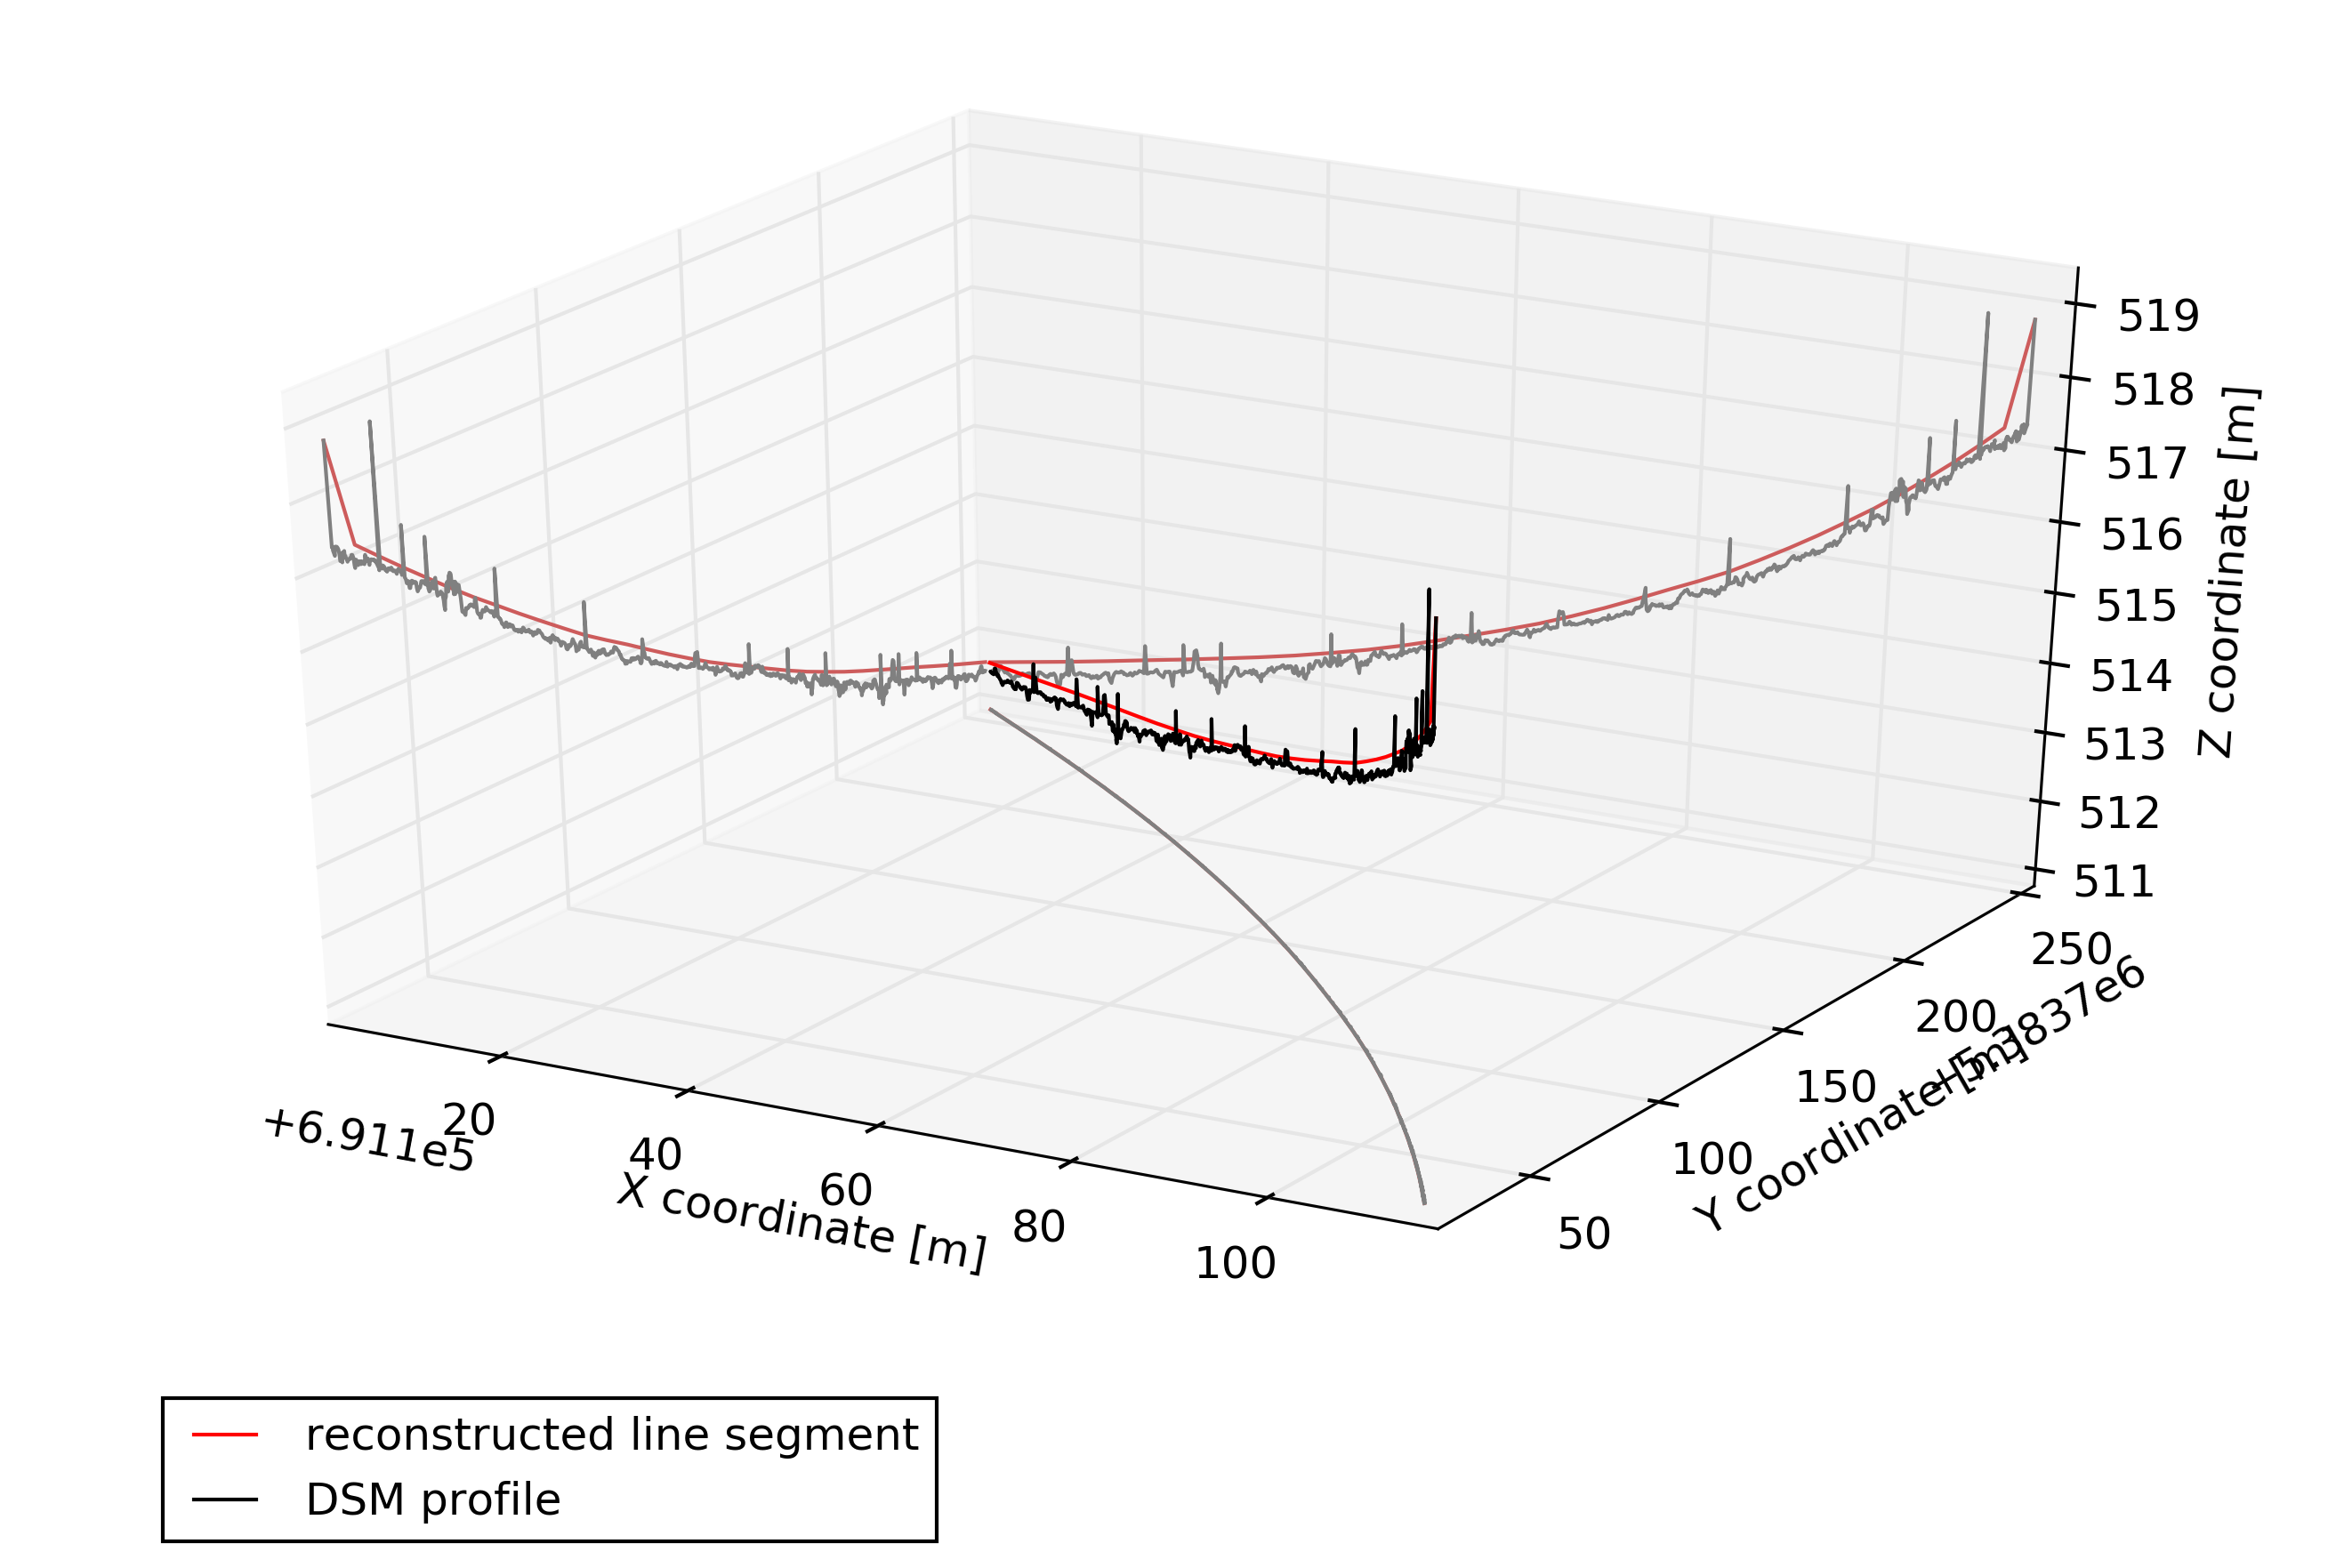
\includegraphics[width=\textwidth]{4_Test_3D.png} %%% 換,字重疊。
  \caption{\small The reconstructed line segments and the unrefined DSM profile in UTM coordinate system (in Zone 32N).}
  \label{fig:Test3D_1}
  \vspace{1cm}
  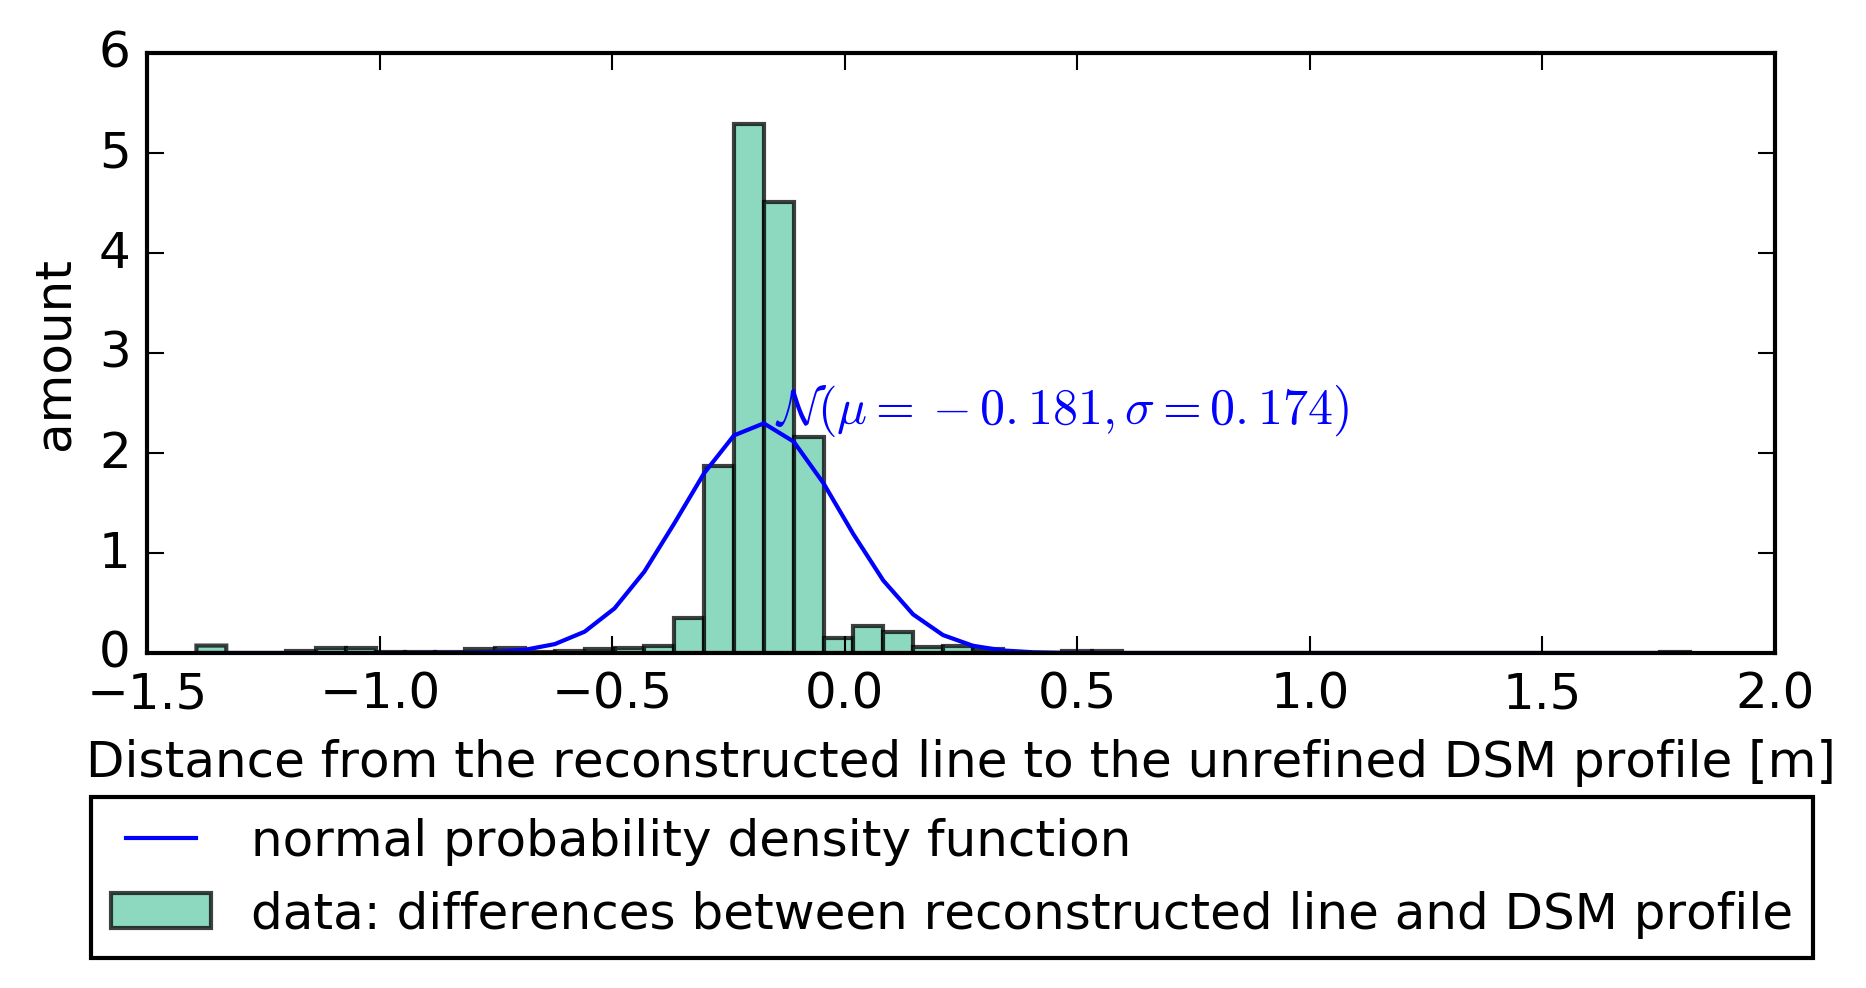
\includegraphics[width=\textwidth]{4_Test_hist.png} %%% 換,字太小、xlim。
  \caption{\small Histogram of the distances from the reconstructed line to the unrefined DSM profile.}
  \label{fig:TestHist_1}
\end{figure}

\clearpage

Images configuration plays an important roll in 3D reconstruction. %!!! discussion
\cref{fig:TestImgNum_1} shows: when more images cover a line segment, more measurements (extracted line segment) are provided, resulting higher redundancies in LS adjustment. (...???)

Since the estimated variance-covariance matrix of the estimated parameters $\hat{\Sigma}_{\hat{X}\hat{X}}$ depends on both the design matrix $A$ (i.e. the configuration) and the posterior standard deviation $\hat{\sigma}_0$ (i.e. the posterior measurements quality):
\begin{equation}
\hat{\Sigma}_{\hat{X}\hat{X}}=\hat{\sigma}_0^2(A^TA)^{-1}=
\begin{bmatrix}
\hat{\sigma}_{\hat{X}}^2 && \hat{\sigma}_{\hat{X}\hat{Y}} && \hat{\sigma}_{\hat{X}\hat{Z}} \\
\hat{\sigma}_{\hat{Y}\hat{X}} && \hat{\sigma}_{\hat{Y}}^2 && \hat{\sigma}_{\hat{Y}\hat{Z}} \\
\hat{\sigma}_{\hat{Z}\hat{X}} && \hat{\sigma}_{\hat{Z}\hat{Y}} && \hat{\sigma}_{\hat{Z}}^2
\end{bmatrix}
\end{equation}
we are not able to tell from the variances $\hat{\sigma}_{\hat{X}}$, $\hat{\sigma}_{\hat{Y}}$, $\hat{\sigma}_{\hat{Z}}$ whether the .

By setting a constant priori standard deviation value in all the LS adjustment processes (i.e. assuming the measurements are of same quality in each segment), the priori variance-covariance matrix of the estimated parameters $\Sigma_{\hat{X}\hat{X}}$ reflects the quality of the design matrix (i.e. the configuration strength) in each LS adjustment processes.
\begin{equation}
\Sigma_{\hat{X}\hat{X}}=\sigma_0^2(A^TA)^{-1}
\end{equation}

\cref{fig:TestdesignHV_1} shows:


\begin{figure}
  \centering
  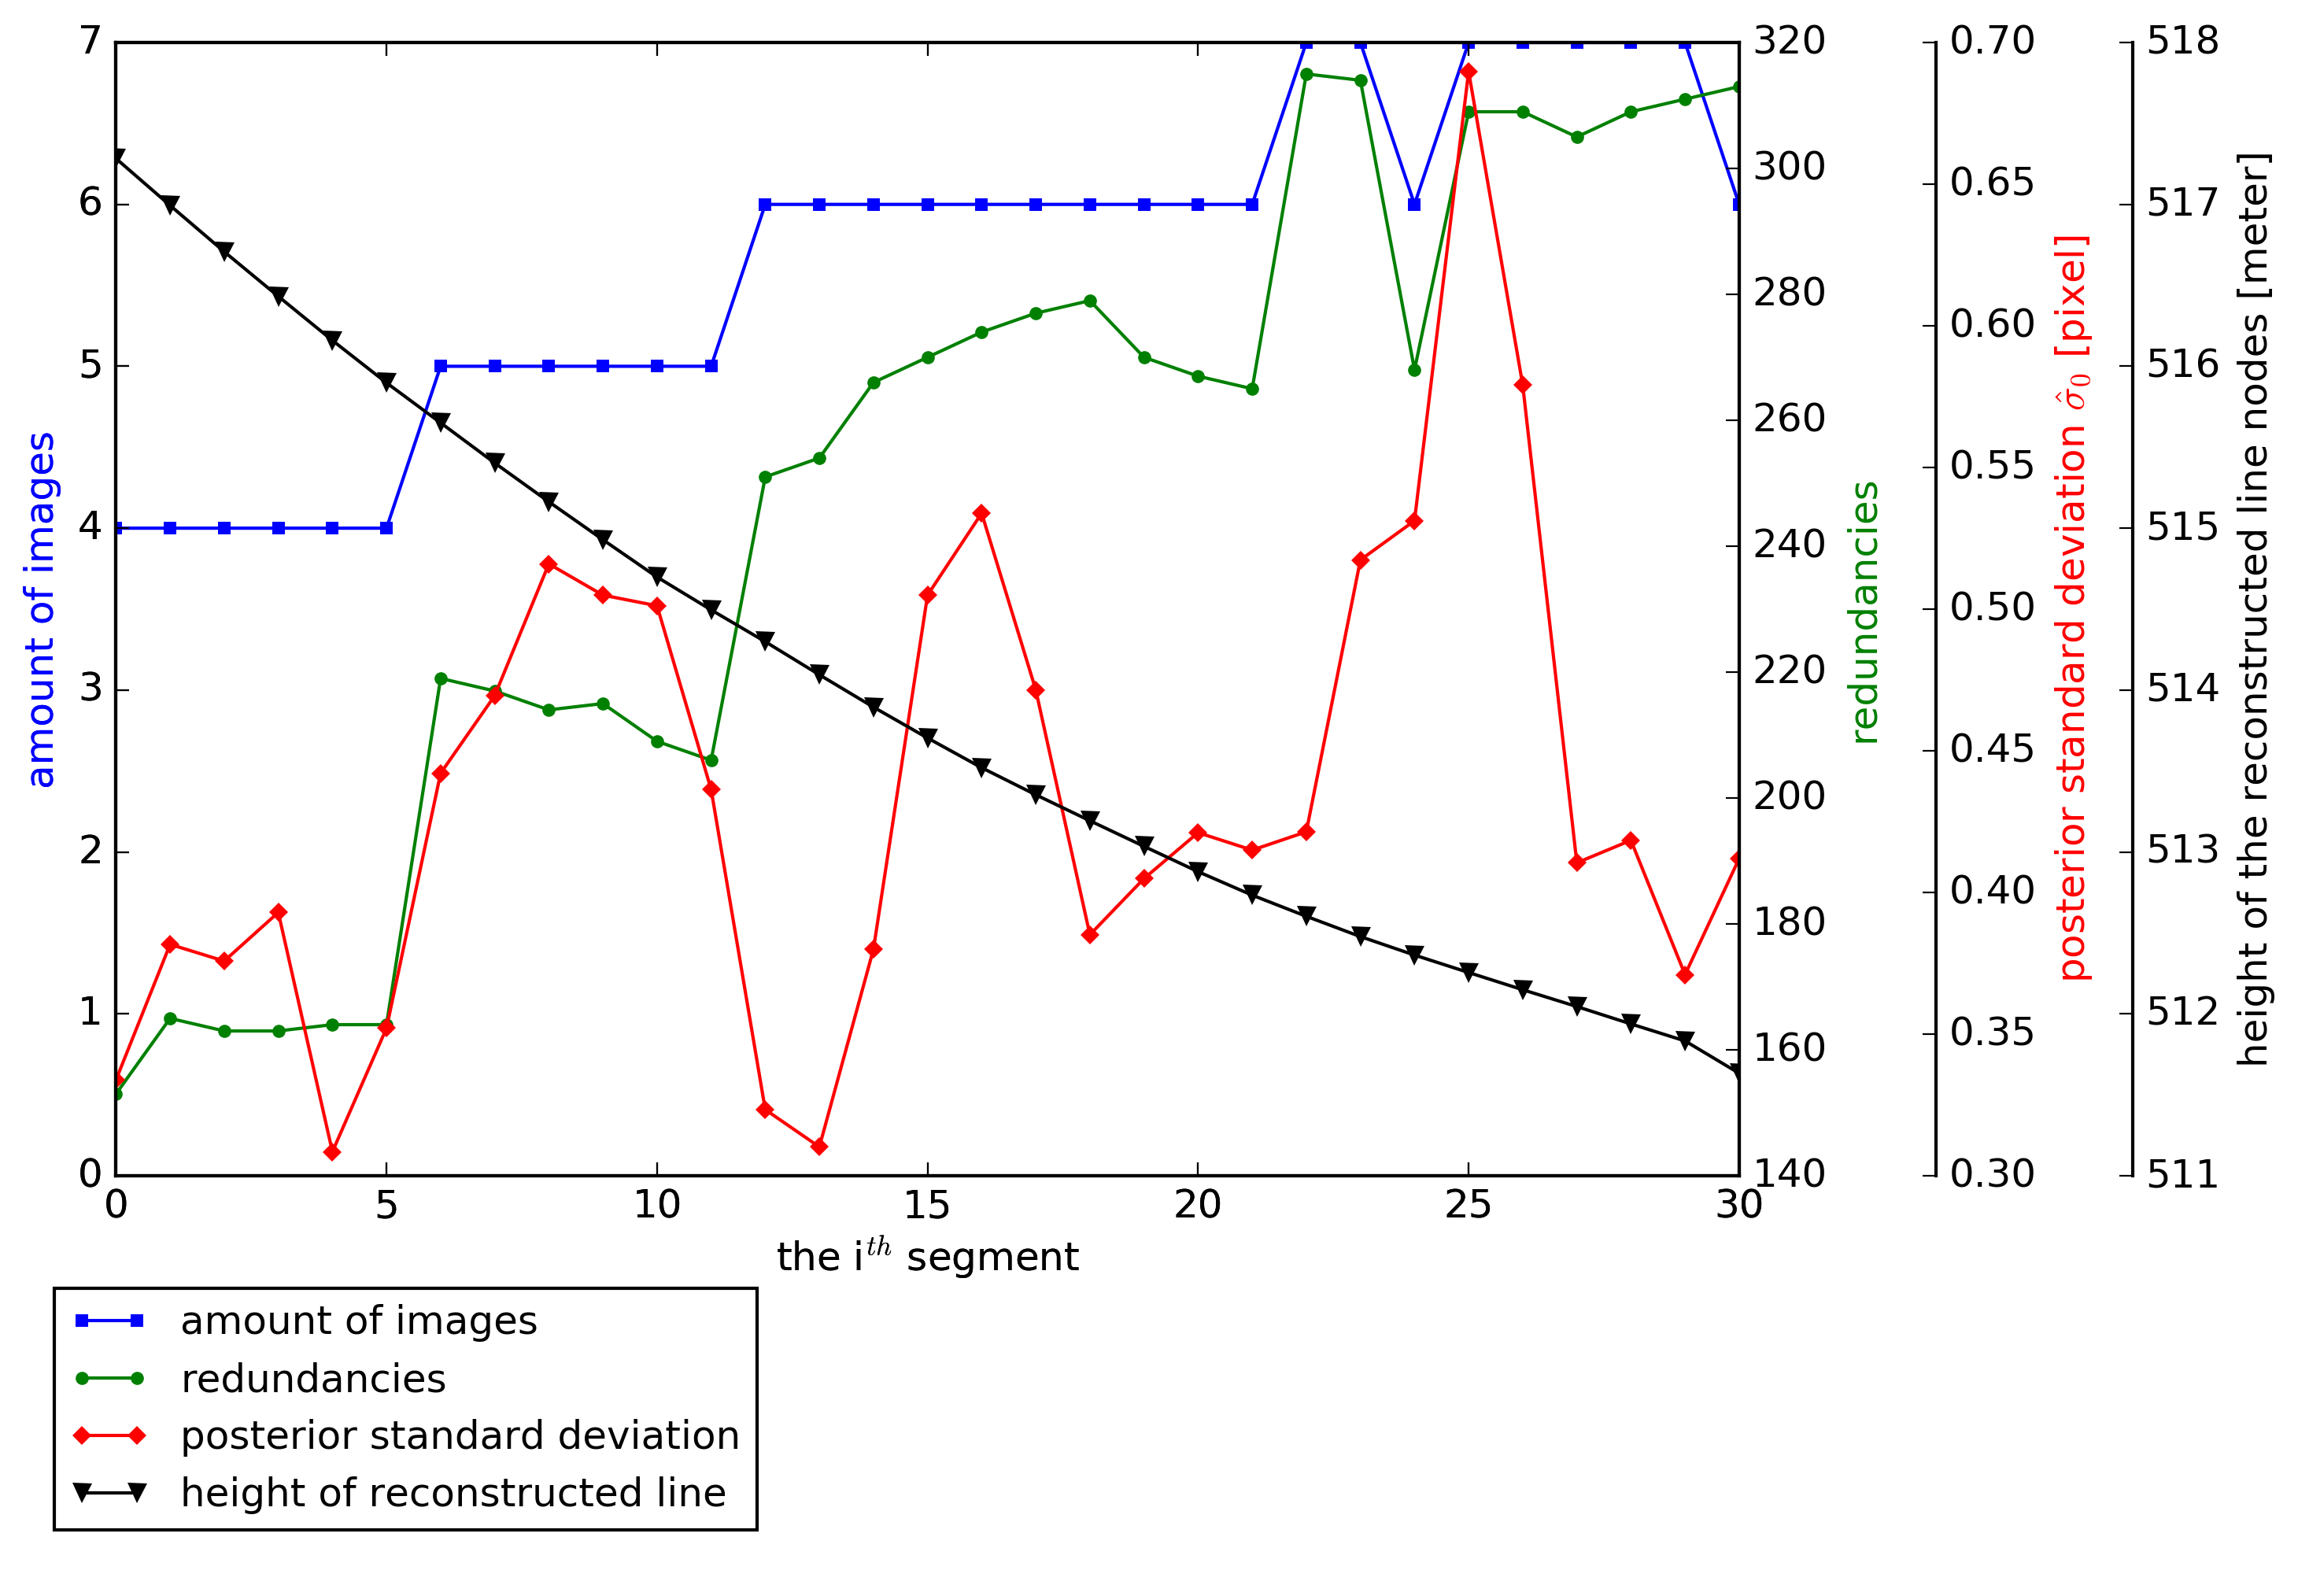
\includegraphics[width=0.95\textwidth]{4_Test_ImgNum.png} %%% 換,字重疊。
  \caption{\small The relationship between image amount, the resulting reconstructed line segments, and the redundancies and posterior standard deviation in LS adjustment.}
  \label{fig:TestImgNum_1}
  \vspace{1cm}
  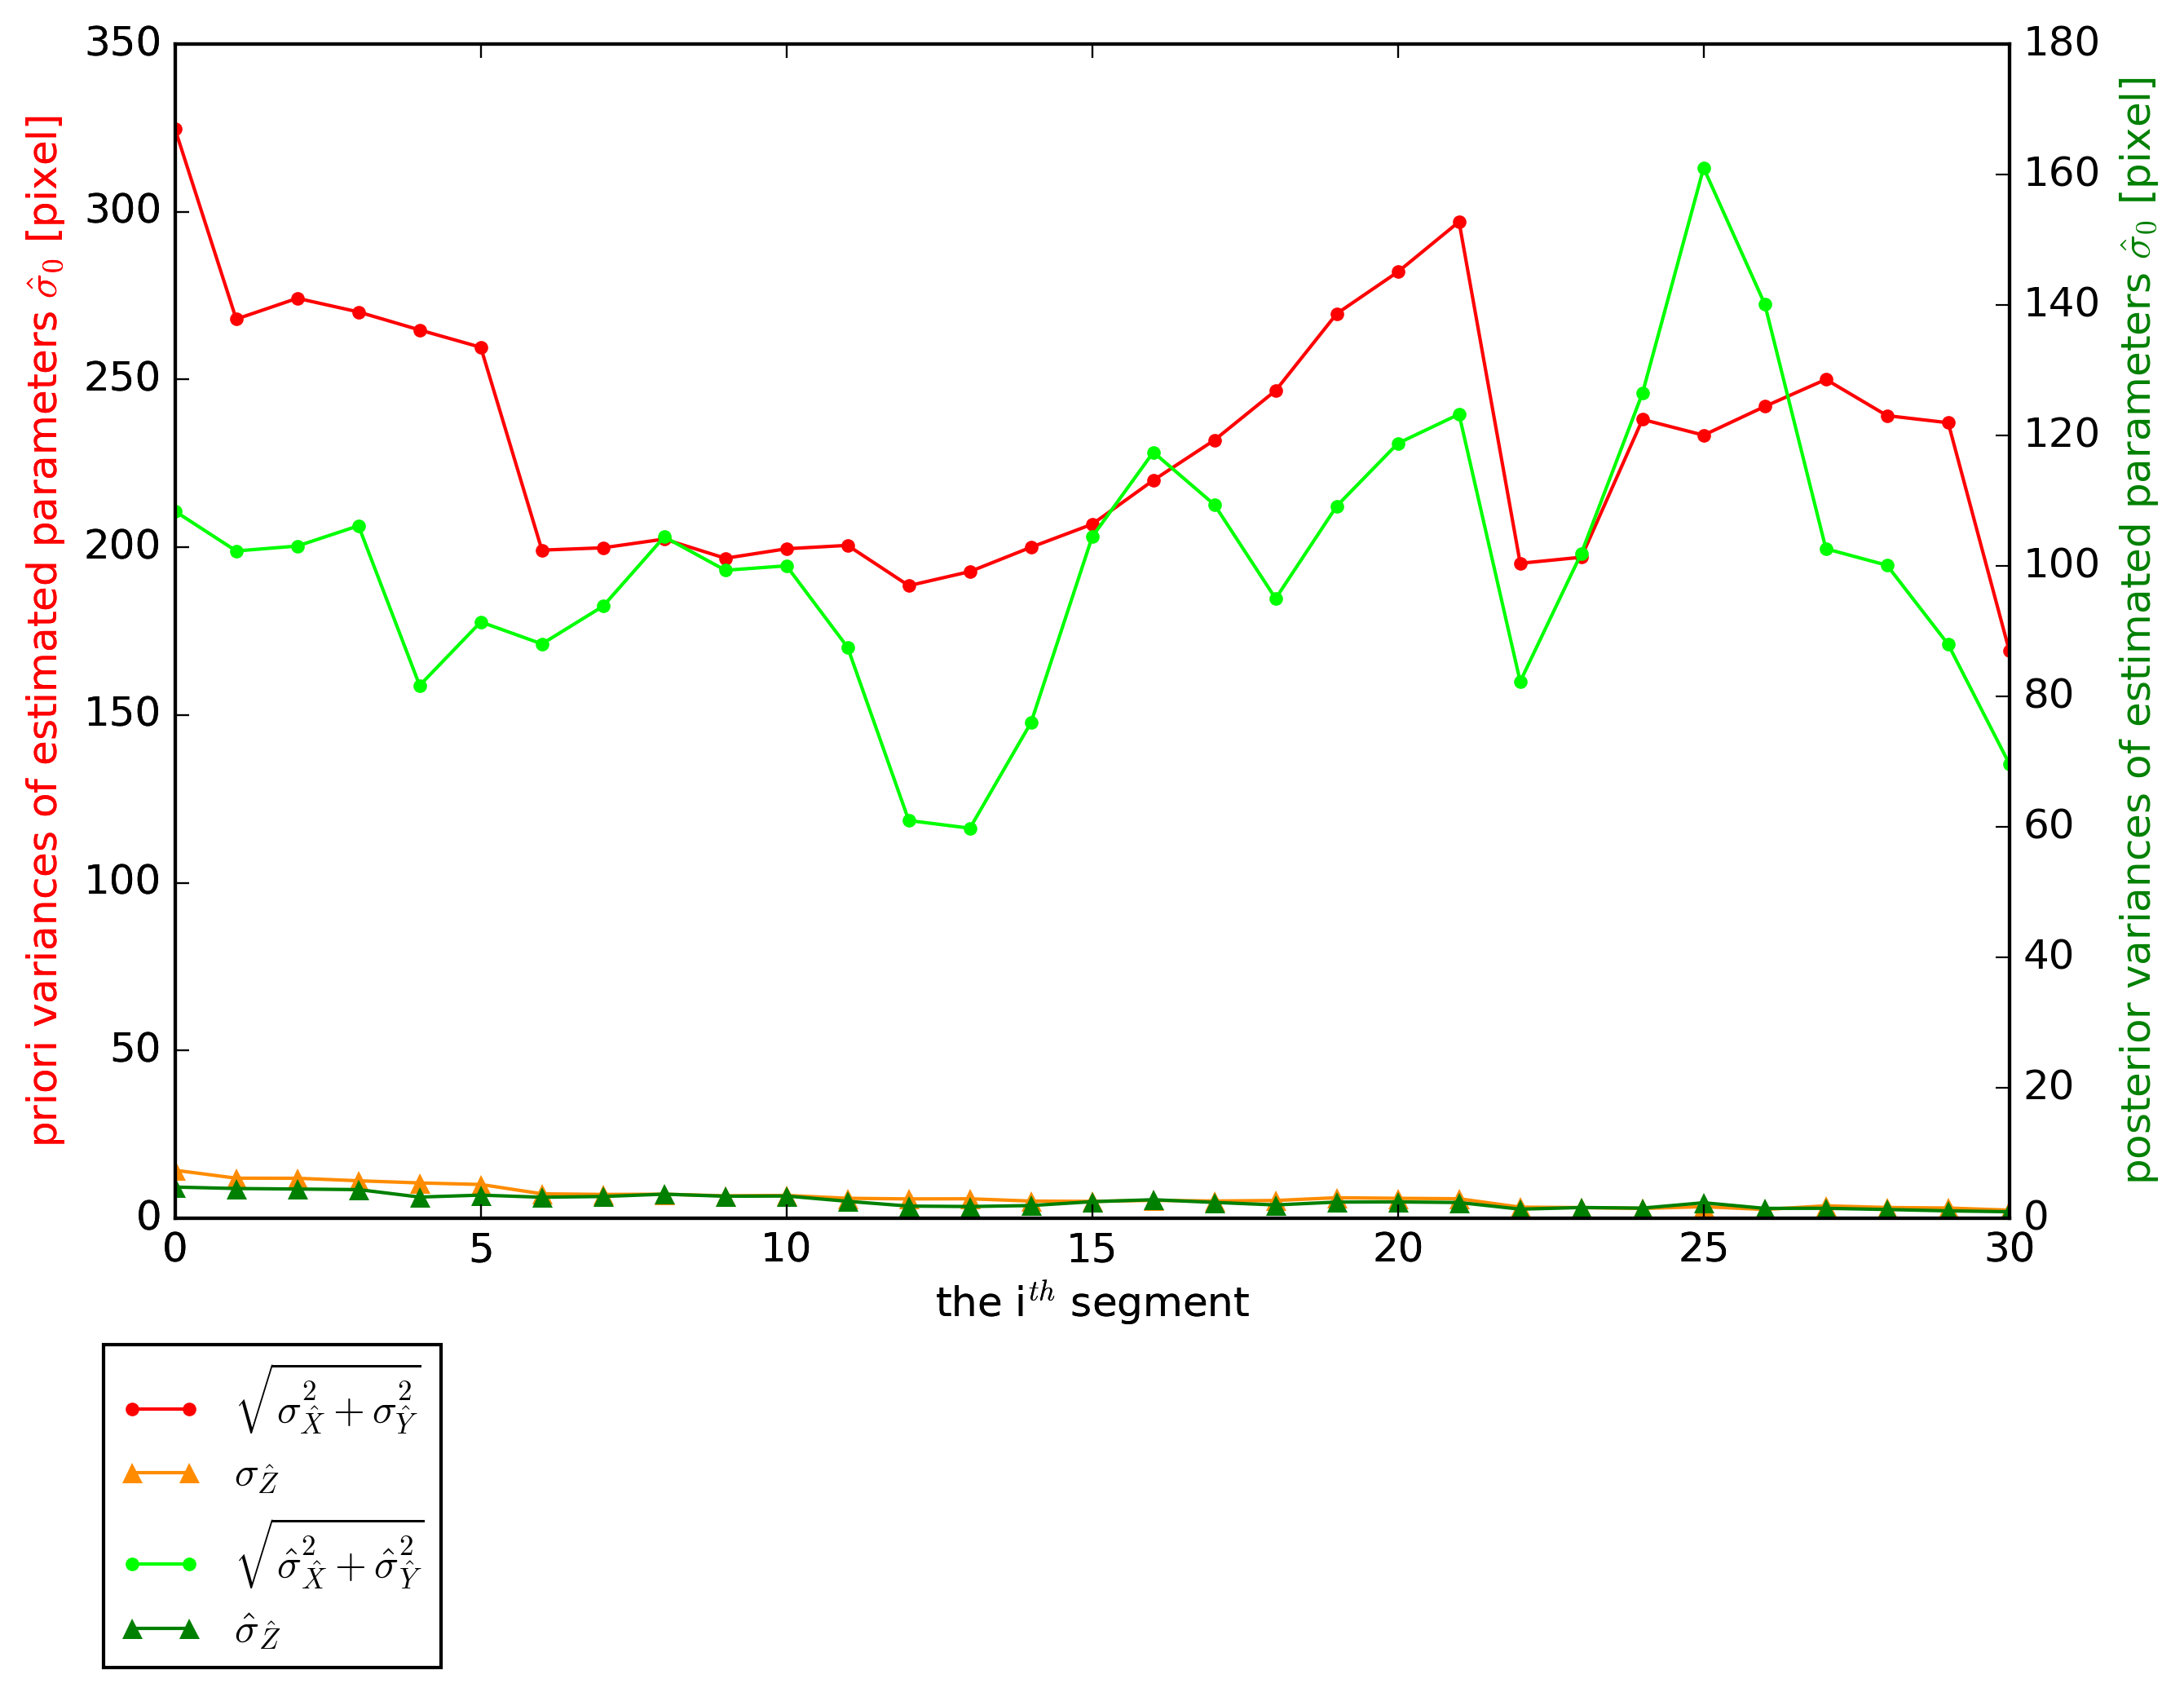
\includegraphics[width=0.8\textwidth]{4_Test_design_XY_Z.png} %%% 換,字太小、xlim。
  \caption{\small The variances of the estimated object coordinates, in horizontal and vertical directions, for both priori and posterior.}
  \label{fig:TestdesignHV_1}
\end{figure}


\clearpage

%\subsection{True Data Result: case2-5}
%\label{sec:trueresult-3}




%%%%%%%%%%%%%%%%%%%%%%%%%%%%%%%%%%%%%%%%%%%%%%%%%%%%%%%%
\section{Discussion: Influence of the Image Distribution and Amount}
\label{sec:discussion-ImageDistributionAmount}




%%%%%%%%%%%%%%%%%%%%%%%%%%%%%%%%%%%%%%%%%%%%%%%%%%%%%%%%
%3.1  Reference Data
%The primary reference dataset used in this paper is a 3D point cloud acquired by airborne laser scanning with a density of approximately 0.5 points per square meter.  The laser point cloud data is georeferenced in UTM Zone 31 North, ETRS89 and contains orthometric heights with respect to EGM 2008.  The orthometric  heights  were  converted  to  ellipsoidal  heights  by  simply dding the undulations from EGM 2008.  Only the first pulse returns is used in this study, as the DSM produced by image matching corresponds to the visible surface.  The LIDAR data for the errassa and Vacarisses test areas was acquired on 26th and 27th ovember 2007. The LaMola LIDAR data was acquired on 26th ovember 2007 and 4th May 2008

%%%%%%%%%%%%%%%%%%%%%%%%%%%%%%%%%%%%%%%%%%%%%%%%%%%%%%%%
4.3 Internal Factors

4.3.1 Correctness of

4.3.2 Verification of

4.3.3 Precision of


%%%%%%%%%%%%%%%%%%%%%%%%%%%%%%%%%%%%%%%%%%%%%%%%%%%%%%%%
4.4 External Factors

4.4.1 Influence of 

%noch etwas Fülltext
%\blinddocument
